% \documentclass[a4paper,10pt]{article}
% \usepackage[utf8]{inputenc}
% \usepackage{fullpage}
% \usepackage{graphicx} % pour insérer des images
% \usepackage{epstopdf}
% % Les N, Z..., math quoi
% \usepackage{amsthm}
% \usepackage{amsmath}
% \usepackage{stmaryrd}
% \usepackage{amsfonts}
% \usepackage{tikz}
% \usepackage{tikz-qtree}
% % les figure imbriquées
% \usepackage{epsfig}
% \usepackage{subfigure}
% \usepackage[francais]{babel}
% \usepackage[algoruled,french,onelanguage]{algorithm2e}


% %opening
% \title{}
\itodo{sg induit -> sg engendré ?}
\itodo{Notations G, p, T ?? + refaire la complexité en conséquence}
\itodo{justifier W=12..24 ?}

Nous avons vu au chapitre précédent que l'analyse morphologique fonctionne par comparaison des graphes de flot de contrôles.
Dans ce chapitre nous formalisons le fonctionnement du détecteur par analyse morphologique et nous nous intéressons au problème de la détection d'isomorphismes de sous-graphes. 
Nous définissons ce qu'est un graphe de flot, notion plus spécifique que la notion générale de graphe, au sein duquel les fils d'un sommet sont ordonnés.
Cette restriction rend le problème de la recherche d'isomorphisme de sous-graphes de flot résoluble \todo{typo?} en temps polynômial alors qu'il est NP complet \todo{typo?} dans le cas général.

\section{Analyse d'un détecteur par analyse morphologique}
\subsection{Graphes de flot}
Nous avons vu que les graphes de flot de contrôle sur lesquels nous travaillons sont étiquetés (définition \ref{def:graphe-oriente}) et, une fois réduits, les étiquettes possibles sont les suivantes : $INST$, $JMP$, $JCC$, $CALL$, $RET$, $HLT$ et $UNDEF$.
Le nombre de fils d'un sommet est sa valence (définition \ref{def:valence}) ; à chaque étiquette est associée une valence maximale. Par exemple les instructions de saut conditionnel $JCC$ ont au maximum deux successeurs.

\begin{defi}
Un graphe orienté et étiqueté $T=(V, L, l, E)$ est composé par les ensembles finis V, L, E, et la fonction totale $l:V\rightarrow L$.
V est l'ensemble des sommets de T, L un ensemble d'étiquettes, l la fonction donnant l'étiquette d'un sommet, et $E\subset V\times V$ est l'ensemble des arcs de T tel que $(t, h)\in E$ ssi il y a un arc entre le sommet t et le sommet h.
\label{def:graphe-oriente}
\end{defi}

\begin{defi}\label{def:valence}
 La valence d'un sommet d'un graphe est le nombre de fils de ce sommet.
\end{defi}


Afin de refléter l'incomplétude des graphes de flot de contrôles reconstruits, les graphes sur lesquels nous sommes amenés à travailler peuvent être partiels : il y a des branches qui peuvent être inconnues.
Par exemple un sommet d'étiquette $JCC$ ayant un seul fils est incomplet : la cible du saut est inconnue.
% De plus pour simplifier les algorithmes impliqués dans la recherche de parties communes à plusieurs graphes, il est pratique de forcer les fils de chaque sommet à être ordonnés.
Nous forçons les fils de chaque sommet à être ordonnés. Il s'agit d'une contrainte forte qui permet de réduire grandement la complexité des algorithmes mis en \oe uvre pour résoudre l'isomorphisme de sous-graphe.
Nous définissons ainsi formellement un graphe de flot à la définition \ref{def:gf}.
Un exemple de graphe de flot est donné en figure \ref{fig:am_exemple_gf}.

\begin{defi}\label{def:gf}
Un graphe de flot est un graphe orienté et étiqueté vérifiant :
\begin{enumerate}
%  \item Chaque sommet a une étiquette, et
%  \begin{enumerate}
%   \item La valence d'un sommet est son nombre de fils
\item On associe à chaque étiquette une arité dans $\mathbb{N}$ : il s'agit de la valence maximale pour tous les sommets ayant cette étiquette, et
%   \item L'arité associée à une étiquette est la valence maximale pour les sommets ayant cette étiquette, et
%  \end{enumerate}
 \begin{enumerate}
  \item Si la valence de chaque sommet est égale à l'arité de son étiquette, le graphe de flot est dit complet
  \item Dans le cas contraire, il s'agit d'un graphe de flot incomplet
 \end{enumerate}
 \item Les fils de chaque sommet sont ordonnés : les arcs ont pour label l'ordre i du fils (où i est un entier compris entre 1 et la valence du sommet)\\
       L'ensemble des arcs est $E\subset V\times \mathbb{N}\times V$ tel que $(t, i, h)\in E$ ssi il y a un arc numeroté i entre le sommet t et le sommet h.
%  \item La valence de ses sommets est bornée
\end{enumerate}
\end{defi}

% On dispose d'un corpus de programmes malveillant. Le graphe de flot de chaque programme malveillant a été déterminé et on a découpé
% On cherche à identifier les graphes de flot du corpus qui seraient présents dans le graphe de flot de test T à analyser.


% On cherche à identifier des parties d'un graphe de flot inconnu qui seraient présentes dans une collection de graphes de flots de contrôles donnée (corpus de logiciels malveillants par exemple).
% On note T le graphe de flot de test à analyser.
% On définit formellement la reconnaissance de deux parties communes dans deux graphes par l'existence d'un isomorphisme de sous-graphe entre un graphe du corpus et T.

% \begin{figure}[h]
% \begin{center}
% \def\imagetop#1{\vtop{\null\hbox{#1}}}
% \begin{tabular}[t]{|c|c|}
% \hline
% Graphe de flot de contrôle réduit & Graphe de flot\\
% \hline
% \imagetop{\includegraphics[width=0.2\textwidth]{supports/detection/detectionNGF_cropped10.pdf}}
% &
% \imagetop{\includegraphics[width=0.2\textwidth]{supports/detection/detectionGF_cropped10.pdf}}
% \\
% \hline
% \end{tabular}
% \end{center}
% \caption{Transformations du graphe de flot de contrôle de l'exemple de la figure \ref{fig:am_prog}}
% \label{fig:am_cfg_gf}
% \end{figure}

\begin{figure}[h]
\begin{center}
\includegraphics[width=0.13\textwidth]{supports/detection/detectionGF_cropped0.pdf}
\end{center}
\caption{Exemple de graphe de flot}
\label{fig:am_exemple_gf}
\end{figure}

% Un graphe de flot (définition \ref{def:gf}) est un graphe orienté particulier.

% Le point 1 force à expliciter les fils ; par exemple un \emph{JCC} a nécessairement deux successeurs, selon que la condition vérifiée est satisfaite ou non. Les sites incomplets sont une extension autorisant que certains fils ne soit pas connus (on peut les omettre dans la représentation ou ajouter un fils artificiel $\bot$).
% Le point 2 est une restriction forte utilisée pour rendre la détection possible en un temps raisonnable.

\subsection{Isomorphisme de graphes et de sous-graphes de flot}
Deux graphes de flot sont isomorphes s'ils vérifient les
propriétés de la définition \ref{def:iso-go}, c'est à dire s'il existe une permutation des sommets de l'un tel que le graphes modifié soit structurellement identique au second.

\begin{defi}\label{def:iso-go}
Soit $T=(V_T, L_T, l_T, E_T)$ et $P=(V_P, L_P, l_P, E_P)$ deux graphes de flot. Ils sont dits isomorphes s'il existe une bijection $f:V_T\rightarrow V_P$ entre les sommets de T et ceux de P et
si f préserve la structure d'adjacence des graphes avec l'ordre des fils, c'est à dire si \\
$\forall u, v \in V_T$ et $i\in\mathbb{N} : (u, i, v) \in E_T \Leftrightarrow (f(u), i, f(v)) \in E_P$.
\end{defi}

On définit le sous-graphe d'un graphe T selon la définition \ref{def:sousgrapheflot} et le sous-graphe de flot induit par un ensemble de sommet en définition \ref{def:sousgrapheflot-induit}.

\begin{defi}\label{def:sousgrapheflot}
Un graphe de flot $P=(V_P, L_P, l_P, E_P)$ est un sous-graphe du graphe de flot $T=(V_T, L_T, l_T, E_T)$ si et seulement si $V_P \subset V_T$, $E_P\subset\{(t, i, h)\in E_T / t, h \in V_P \}$, et $\forall u\in V_P, l_P(u)=l_T(u)$
\end{defi}

\begin{defi}\label{def:sousgrapheflot-induit}
Le sous-graphe induit d'un graphe de flot $T=(V_T, L_T, l_T, E_T)$ à partir de l'ensemble de sommets $V_P \subset V_T$ est le graphe de flot $P=(V_P, L_P, l_P, E_P)$ tel que $E_P=\{(t, i, h)\in E_T / t, h \in V_P \}$, $L_P=L_T$, et $l_P=l_{T\vert V_P}$.
\end{defi}

% il est
% important de noter qu'un sous-graphe a des sommets pris arbitrairement au graphe de base mais que ses arcs sont exactement tous ceux
% du graphe de base qui s'appliquent aux sommets choisis. 
% Notre problème
% consiste donc, à partir du graphe de flot T à analyser, à déterminer si un de ses sous-graphes est isomorphe à un des graphes de flot de la base.
Notre problème consiste donc, à partir d'un graphe de flot P connu et d'un graphe de flot T à analyser, à déterminer si P est isomorphe à un sous-graphe de flot de T.
Par exemple sur la figure \ref{fig:ex-gf-sous-gf}, le graphe P est isomorphe au sous-graphe de T induit par les sommets $\{d, e, a\}$ comme à celui formé induit par les sommets sommets $\{b, d, a\}$.


\begin{figure}[ht]
\begin{center}
  \subfigure[Graphe de flot T]{
\label{fig:ex-gf}
% \epsfig{figure=images/def-graphe2.pdf,height=3.5cm}}\quad
% \epsfig{figure=supports/algos/gTGF_circo_cropped0.pdf,height=3.2cm}
\includegraphics[width=0.4\textwidth]{supports/algos/gTGF_circo_cropped0.pdf}
}\quad
  \subfigure[Graphe de flot P, isomorphe à un sous-graphe de T]{
\label{fig:ex-sous-gf}
% \epsfig{figure=images/def-graphe1.pdf,height=3cm}}\\
% \epsfig{figure=supports/algos/gPGF_circo_cropped0.pdf,height=2.5cm}
\includegraphics[width=0.22\textwidth]{supports/algos/gPGF_circo_cropped0.pdf}
}\\
\end{center}
\caption{Exemple de graphe de flot et d'un sous-graphe}
\label{fig:ex-gf-sous-gf}
\end{figure}

\subsection{Sites}
L'analyse morphologique \cite{BKM08} ne cherche pas directement à savoir si un programme malveillant est un sous-graphe du programme analysé ou inversement. 
Cette approche est vouée à l'échec puisqu'une modification mineure de l'un des deux conduirait à une non détection.
Au contraire on va découper les graphes de flot du corpus en sous-graphes tout en gardant le graphe de test T intact.
On cherchera alors des isomorphismes de sous-graphes entre chaque petit graphe de la base et un sous-graphe du graphe de flot de test.

En pratique on va générer un certain nombre de sous-graphes, appelés sites, du corpus de graphes de flot qui seront les motifs que l'on cherche à retrouver dans le graphe de flot analysé : on notera généralement P un graphe de motif. 
Ces sous-graphes sont définis par le sous-graphe induit par les sommets parcourus avec d'un parcours en largeur limité à un certain nombre de sommets, que l'on notera W (typiquement entre 12 et 24), à partir de chaque sommet du graphe d'origine. Ils ont donc une racine qui est le sommet à partir duquel ils ont été générés.

Ainsi un site est un graphe de flot ayant une racine (définition \ref{def-site}). Un site peut être un sous-graphe d'un graphe de flot (définition \ref{def-soussite}) comme dans l'exemple de la figure \ref{fig:ex-gf-site} : le sous-site est généré à partir du sommet $b$ en construisant le sous-graphe induit par les trois premiers sommets atteignables par un parcours en largeur.

\begin{defi}\label{def-site}
Un site P est un graphe de flot ayant une racine : un sommet à partir duquel on peut atteindre n'importe quel autre sommet de P
\end{defi}

\begin{defi}\label{def-soussite}
On appelle sous-site d'un graphe de flot $T$ tout site étant un sous-graphe de $T$.
\end{defi}

\begin{figure}[ht]
\begin{center}
  \subfigure[Graphe de flot T]{
\label{fig:ex-gf}
% \epsfig{figure=images/def-graphe2.pdf,height=3.5cm}}\quad
% \epsfig{figure=supports/algos/c_gTGF.pdf,height=3.5cm}
\includegraphics[width=0.4\textwidth]{supports/algos/gTGF_circo_cropped0.pdf}
}\quad
  \subfigure[Site P, de racine b, isomorphe à un sous-graphe de T]{
\label{fig:ex-site}
% \epsfig{figure=images/def-graphe1.pdf,height=3cm}}\\
% \epsfig{figure=supports/algos/c_gPsite.pdf,height=3cm}
\includegraphics[width=0.3\textwidth]{supports/algos/gPsite_circo_cropped0.pdf}
}\\
\end{center}
\caption{Exemple de graphe de flot et d'un sous-site}
\label{fig:ex-gf-site}
\end{figure}

Générer les site de manière homogène, toujours à l'aide d'un parcours en largeur de taille fixe, permet d'obtenir automatiquement des signatures pour les programmes du corpus.
Nous choisissons le parcours en largeur parce qu'il donne rapidement une structure au site construit tandis qu'un parcours en profondeur donne souvent de longs chemins sans branchements, par exemple.
L'algorithme \ref{algo:generation_site_largeur} détermine, s'il existe, le site d'un graphe de flot généré par parcours en largeur à partir d'un sommet spécifié et limité à un certain nombre de sommets. L'algorithme \ref{algo:generation_sites_largeur} donne l'ensemble des sites d'un graphe de flot obtenus par parcours en largeur limité à un W sommets.

\begin{algorithm}[h]
\DontPrintSemicolon
\caption{Site obtenu par parcours en largeur limité à partir d'un sommet particulier}
\SetAlgoLined
\KwData{Un graphe de flot G, un sommet R de G, un entier W}
\KwResult{Le site, s'il existe, ayant W sommets construit par parcours en largeur à partir du sommet R de G}
\SetKwProg{Fn}{}{}{}
\SetKwFunction{FRecurs}{site}
\Fn(){\FRecurs{G, R, W}}{
$E\leftarrow \emptyset$  \tcc*{E contient les sommets du futur site}
$M\leftarrow \emptyset$  \tcc*{Les sommets visités seront ajoutés à M}
$L\leftarrow$ pile vide  \tcc*{L : file d'attente pour les sommets à visiter}
L.empiler(R)             \\
\While{$|E|<W$ et $L\ne \emptyset$}{
  s $\leftarrow$ L.dépiler()  \\
  $E\leftarrow E\cup {s}$      \\
  $M\leftarrow M\cup {s}$      \\
  \ForEach{f fils de s}{
    \If{$f \notin M$}{
      L.empiler(f)  \\
      $M\leftarrow M\cup {f}$      \\
    }
  }
}
\eIf {$|E|=W$}{
\Return{le sous-site de G induit par les sommets présents dans E, de racine R}
}
{
\Return {FAIL}
}
}
\label{algo:generation_site_largeur}
\end{algorithm}

\begin{algorithm}[h]
\DontPrintSemicolon
\caption{Sites obtenus par parcours en largeur limité}
\SetAlgoLined
\KwData{Un graphe de flot G, un entier W}
\KwResult{L'ensemble de sites ayant W sommets construits par parcours en largeur à partir de chaque sommet de G}
\SetKwProg{Fn}{}{}{}
\SetKwFunction{FRecurs}{sites}
\Fn(){\FRecurs{G, W}}{
$E\leftarrow\emptyset$\\
\ForEach {s sommet de G}{
  $S \leftarrow site(G, s, W)$\\
  \If{S $\ne$ FAIL}{
    $E=E\cup\{S\}$
  }
  \Return{E}
}
}
\label{algo:generation_sites_largeur}
\end{algorithm}

\paragraph{Complexité.}
Calculons la complexité de l'obtention d'un site par parcours en largeur limité à W sommets en prenant en compte le nombre d'opération de dépilement ou d'empilement dans la file L.
Nous avons vu \todo{vrai?} que chaque sommet a au plus $k$ fils.
De plus le parcours s'arrête dès que W sommets ont été ajoutés à l'ensemble E. Il peut arriver que les fils du $W^e$ sommet soient ajoutés à la liste d'attente (mais ils ne seront pas ajoutés à E).
Dans le pire des cas on empile donc la racine puis $k$ fils pour $W$ sommets et on dépile $W$ sommets. La complexité de l'algorithme \ref{algo:generation_site_largeur} est donc $O((k+1).W)$.

L'algorithme \ref{algo:generation_sites_largeur} itère l'opération précédente sur les $n_G$ sommets du graphe G : sa complexité est  $O(n_G.(k+1).W)$.

% \begin{defi}\label{def-site-incomplet}
% Un site incomplet est un site dans lequel certains n\oe uds n'ont pas le bon nombre de fils mais ces fils sont tout de même ordonnés.
% \end{defi}

\subsection{Fonctionnement d'un détecteur morphologique \label{sec:detecteur_morphologique}}
Nous avons à présent tous les éléments nécessaires à une définition précise de la méthode de détection par analyse morphologique.

\subsubsection{Constitution des signatures et du corpus}
Nous cherchons à construire un corpus contenant les signatures d'un programme malveillant.
La signature d'un programme malveillant est un ensemble de sites extraits du graphe de flot de ce programme.
Afin que les signatures soient extraites automatiquement nous cherchons donc à construire tous les sites de taille limitée, par parcours en largeur à partir de chaque sommet du graphe de flot.
Un exemple de signature du graphe de flot précédent est donné en figure \ref{fig:gfc_gf_sites}. Nous avons pris, pour l'exemple, des sites de taille 3, bien qu'en réalité nous prenions des sites de taille 24.

\begin{figure}[h]
\begin{center}
\def\imagetop#1{\vtop{\null\hbox{#1}}}
\begin{tabular}[t]{|c|c|}
\hline
Graphe de flot & Signature : ensemble de sites\\
% \hline
\imagetop{\includegraphics[width=0.25\textwidth]{supports/algos/g1gf_cropped10.pdf}}
&
\imagetop{\includegraphics[width=0.6\textwidth]{supports/algos/g1_sites_cropped10.pdf}}
% &
% \imagetop{\includegraphics[width=0.2\textwidth]{supports/algos/g1_prof_cropped10.pdf}}
\\
\hline
\end{tabular}
\end{center}
\caption{Graphe de flot d'un programme et sa signature dans le corpus}
\label{fig:gfc_gf_sites}
\end{figure}

\begin{figure}[h]
\begin{center}
\scalebox{1}{
\begin{tikzpicture}[->,scale=1,>=stealth',thick]%
\node[state, text width=1.1cm, minimum size=1.2cm] (S11){Site 1};
\node[state, right=0.05cm of S11.east, anchor=west, text width=1.1cm, minimum size=1.2cm] (S12){Site 2};
\node[state, below=0.05cm of S11.south, anchor=north, text width=1.1cm, minimum size=1.2cm] (S13){Site 3};
\node[state, right=0.05cm of S13.east, anchor=west,text width=1.1cm, minimum size=1.2cm] (S1p){...};
\node [fit={($(S11.north west) + (0.0, 0.0)$) ($(S1p.south east) + (0.0, 0.0)$)}, draw, dash pattern=on \pgflinewidth off 2pt, label=Programme 1](M1) {};

\node[state, right=1cm of S12.east, anchor=west, text width=1.1cm, minimum size=1.2cm] (S21){Site 1};
\node[state, right=0.05cm of S21.east, anchor=west, text width=1.1cm, minimum size=1.2cm] (S22){Site 2};
\node[state, below=0.05cm of S21.south, anchor=north, text width=1.1cm, minimum size=1.2cm] (S23){Site 3};
\node[state, right=0.05cm of S23.east, anchor=west,text width=1.1cm, minimum size=1.2cm] (S2p){...};
\node [fit={($(S21.north west) + (0.0, 0.0)$) ($(S2p.south east) + (0.0, 0.0)$)}, draw, dash pattern=on \pgflinewidth off 2pt, label=Programme 2](M2) {};

\node[state, right=1cm of S22.east, anchor=west, text width=1.1cm, minimum size=1.2cm] (S31){Site 1};
\node[state, right=0.05cm of S31.east, anchor=west, text width=1.1cm, minimum size=1.2cm] (S32){Site 2};
\node[state, below=0.05cm of S31.south, anchor=north, text width=1.1cm, minimum size=1.2cm] (S33){Site 3};
\node[state, right=0.05cm of S33.east, anchor=west,text width=1.1cm, minimum size=1.2cm] (S3p){...};
\node [fit={($(S31.north west) + (0.0, 0.0)$) ($(S3p.south east) + (0.0, 0.0)$)}, draw, dash pattern=on \pgflinewidth off 2pt, label=Programme 3](M3) {};

\node[right=1.5cm of S32.south east, anchor=west, text width=1.1cm, minimum size=1.2cm] (Mp){...};

% \node[state, text width=2cm, minimum size=3cm] (TEXT){Code};
% \node[state, below = -3cm of TEXT.north, text width=2cm, minimum size=3cm, anchor=north] (DATA){Données};
% \draw ($(BIN.east) + (0.5, 0) $) -- node[below]{\large Enpaquetage} ($(BIN.east) + (3cm, 0) $);
\node [fit={($(M1.north west) + (0.0, 0.6)$) ($(M3.south east) + (1.0, 0.0)$) ($(Mp.east) + (0.6, 0.0)$)}, draw, label=] {};
\end{tikzpicture}
}
\end{center}
\caption{Corpus pour l'analyse morphologique}
\label{fig:corpus}
\end{figure}



\subsubsection{Détection}
Supposons que l'on dispose du corpus comprenant la signature du programme précédent et du graphe de flot de test, provenant d'un programme à analyser.
Le détecteur morphologique cherche à trouver tous les sites du corpus qui sont des sous-sites du graphe de flot de test et, selon les programmes dans lesquels ils étaient présents, à rapprocher le programme analysé de ceux du corpus.

Prenons le programme de test de la figure \ref{fig:am_exemple_gf_test}.
Le site 1 du corpus (figure \ref{fig:gfc_gf_sites}) est un sous-site de ce graphe de flot : en partant du premier sommet \emph{JCC}, dans les deux cas le fils numéroté 1 est un \emph{CALL} et le fils numéroté 2 est un \emph{JCC}.
De même les sites 3 et 4 sont des sous-sites du graphe de flot de test. Par contre le site 2 n'est pas un sous-site : aucun sommet d'étiquette \emph{CALL} n'a pour fils numéroté 2 un sommet d'étiquette \emph{RET}.


\begin{figure}[h]
\begin{center}
\includegraphics[width=0.25\textwidth]{supports/algos/g1p_cropped10.pdf}
\end{center}
\caption{Graphe de flot d'un programme à analyser}
\label{fig:am_exemple_gf_test}
\end{figure}


\subsection{Problème de la détection des sites isomorphes}
Le problème se pose alors de la manière suivante. On dispose d'une liste de sites et %provenant de multiples graphes de flot de contrôle différents.
on veut déterminer, dans le graphe de flot de test T, les sites qui sont isomorphes à (au moins) un site présent dans la liste connue. 
% Dans une optique de détection, il est aussi nécessaire d'associer chaque site de la base connue au programme dont il est issu.

On a alors trois problèmes successifs, de difficulté croissante et faisant intervenir différents algorithmes.
\begin{pb}\label{pbisog}
 Comment savoir si deux graphes sont isomorphes ?
\end{pb}

\begin{pb}\label{pbisosg}
 À partir d'un site $P$ et d'un graphe de flot $T$, comment savoir si $P$ est un sous-site de $T$ ?
\end{pb}

% Dans le problème~\ref{pbisosg}, on nomme $P$ le site de motif et $T$ le graphe de test.

\begin{pb}\label{pbisosgbase}
%  À partir d'un ensemble de sites $L_P$ et d'un graphe de flot $T$, comment savoir s'il existe $P\in L_P$ tel que $P$ est un sous-site $T$ ?
 À partir d'un ensemble de sites $L_P$ et d'un graphe de flot $T$, comment déterminer l'ensemble des $P\in L_P$ tels que $P$ est un sous-site de $T$ ?
\end{pb}

Dans le cas général, le problème \ref{pbisog} de l'isomorphisme de graphes est connu pour être NP sans que l'on sache s'il est NP complet \cite{Kob94}, tandis que le problème de l'isomorphisme de sous-graphes est NP complet \cite{W05}.
Nous allons présenter quelques approches de ces problèmes et proposer des solutions tirant partie des spécificités des graphes de flot.

Nous verrons que les problèmes de l'isomorphisme de graphes et de sous-graphes de flot sont polynomiaux.
C'est l'utilisation de fils ordonnés pour chaque sommet qui permet de classer ces problèmes dans P.

Nous introduirons dans les deux prochaines sections des approches générales au problème d'isomorphisme de graphes et de sous-graphes puis détaillerons par la suite deux techniques tirant partie des spécificités des graphes de flot et donnant donc une solution accessible en temps polynomial.

\section{Approches générales à l'isomorphisme de sous-graphes}
Nous présentons deux méthodes générales pour la résolution du problème d'isomorphisme de sous-graphes : l'approche matricielle par recherche exhaustive et l'algorithme d'Ullmann. Nous tenterons d'adapter ce second algorithme au problème des graphes de flot.

Dans cette section on traite donc le cas général de l'isomorphisme de graphes et de sous-graphes orientés l'illustre la figure \ref{fig:ex-graphe-sg}. En particulier ces graphes ne sont, sauf mention du contraire, pas étiquetés et les fils des sommets ne sont pas ordonnés.

\begin{figure}[h]
\begin{center}
  \subfigure[Graphe T]{
\label{fig:ex-graphe}
% \epsfig{figure=images/def-graphe2.pdf,height=3.5cm}}\quad
% \epsfig{figure=supports/algos/c_gT.pdf,height=3.5cm}
\includegraphics[width=0.4\textwidth]{supports/algos/gT_circo_cropped0.pdf}
}\quad
  \subfigure[Graphe P, isomorphe à un sous-graphe de T]{
\label{fig:ex-sg}
% \epsfig{figure=images/def-graphe1.pdf,height=3cm}}\\
% \epsfig{figure=supports/algos/c_gP.pdf,height=3cm}
\includegraphics[width=0.2\textwidth]{supports/algos/gP_circo_cropped0.pdf}
}\\
\end{center}
\caption{Exemple de graphe et d'un sous-graphe}
\label{fig:ex-graphe-sg}
\end{figure}

Nous donnons les définitions précédentes de graphes orientés, de sous-graphe et sous-graphe induit ainsi que d'isomorphisme de graphes, dans le cas habituel des graphes orientés quelconques, aux définitions \ref{def:graphe}, \ref{def:sousgraphe}, \ref{def:sousgraphe-induit} et \ref{def:isog}, respectivement.

\begin{defi}\label{def:graphe}
Un graphe orienté $T=(V, E)$ est composé par les ensembles finis V et E.
V est l'ensemble des sommets de T, $E\subset V\times V$ est l'ensemble des arcs de T tel que $(t, h)\in E$ ssi il y a un arc entre le sommet t et le sommet h.
\end{defi}

\begin{defi}\label{def:sousgraphe}
Un graphe orienté $P=(V_P, E_P)$ est un sous-graphe du graphe orienté et étiqueté $T=(V_T, E_T)$ si et seulement si $V_P \subset V_T$ et $E_P\subset\{(t, h)\in E_T / t, h \in V_P \}$.
\end{defi}

\begin{defi}\label{def:sousgraphe-induit}
Le sous-graphe induit d'un graphe orienté et étiqueté $T=(V_T, E_T)$ à partir de l'ensemble de sommets $V_P \subset V_T$ est le graphe $P=(V_P, E_P)$ tel que $E_P=\{(t, h)\in E_T / t, h \in V_P \}$.
\end{defi}

\begin{defi}\label{def:isog}
Soit $T=(V_T, E_T)$ et $P=(V_P, E_P)$ deux graphes orientés. Ils sont dits isomorphes s'il existe une bijection $f:V_T\rightarrow V_P$ entre les sommets de T et ceux de P et si f préserve la structure d'adjacence des graphes, c'est à dire si : $\forall u, v \in V_T, (u, v) \in E_T \Leftrightarrow (f(u), f(v)) \in E_P$.
\end{defi}

\subsection{Représentation sous forme matricielle et recherche exhaustive}
On peut représenter les graphes sous forme de matrices. On définit la matrice d'adjacence M d'un graphe T suivant les arcs qu'il contient si ses sommets sont ordonnés dans $V=\{v_1, v_2, ..., v_n\}$. Ensuite s'il y a un arc du sommet $v_i$ vers le sommet
$v_j~\mbox{alors}~M_{i, j}=~1,~\mbox{sinon}~M_{i,~j}=~0$ (définition \ref{def-adjmatrice}).
Pour un graphe donné dont les sommets ne sont pas ordonnés, on peut choisir arbitrairement un ordre à ses sommets et dans ce cas il y a autant de matrices d'adjacence possibles pour ce graphe qu'il y a de permutations de ses sommets. 

Par la suite la matrice $M_T$ d'adjacence d'un graphe T représente une de ces matrices, arbitrairement fixée à la première occurence de $M_T$.
Le choix d'une matrice d'adjacence n'a pas d'impact sur les solutions trouvées puisque toutes les matrices d'adjacence d'un graphe sont les mêmes à une permutation des sommets près, et, par la suite, nous n'utilisons des égalités entre ces matrices qu'à une permutation près.
% Dans les implémentations il est facile de fixer arbitrairement un ordre aux sommets. 
% En mémoire chaque sommet du graphe est réprésenté par une structure, il suffit de les ordonner selon l'adresse mémoire de cette structure. Enregistrés dans un fichier, les sommets sont décrits un par un, ce qui donne un ordre naturel.

\begin{defi}\label{def-adjmatrice}
Soit T=(V, E) un graphe orienté à $n \in \mathbb{N}$ sommets ordonnés. La matrice d'adjacence M associée à T est la matrice $n \times n$ définie par : 
$M_{i, j} = \left\{
  \begin{array}{ll}
	  1 & si\ (i, j) \in E
	\\0 & \mbox{sinon.}
  \end{array}
\right.
$
\end{defi}

Par exemple, les graphe P et T de la figure \ref{fig:ex-graphe-sg} ont pour matrice d'adjacence les matrices de la figure~\ref{fig:mat-adj}. 

% \begin{figure}[ht]
% \begin{center}
% $M_{i, j} = \begin{array}{r|ccc}  & a & b & c \\ \hline a & 0 & 1 & 1 \\ b & 0 & 0 & 1 \\ c & 0 & 0 & 0 \end{array}$
% \\
% \end{center}
% \caption{Matrice d'adjacence du graphe P}
% \label{fig:mat-adj}
% \end{figure}

\begin{figure}[ht]
\begin{center}
  \subfigure[$M_T$]{
\label{fig:mat-adjT}
$M_{i, j} = \begin{array}{r|ccccc}  & a & b & c & d & e \\ \hline a & 0 & 0 & 0 & 0 & 0 
							\\ b & 1 & 0 & 0 & 1 & 0
							\\ c & 0 & 0 & 0 & 0 & 0
							\\ d & 1 & 0 & 0 & 0 & 1
							\\ e & 1 & 0 & 1 & 0 & 0
 \end{array}$}\quad
  \subfigure[$M_P$]{
\label{fig:mat-adjP}
$M_{i, j} = \begin{array}{r|ccc}  & \alpha & \beta & \gamma \\ \hline \alpha & 0 & 0 & 0 \\ \beta & 1 & 0 & 1 \\ \gamma & 1 & 0 & 0 \end{array}$}\\
\end{center}
\caption{Matrices d'adjacence des graphes T et P}
\label{fig:mat-adj}
\end{figure}

Le problème de l'isomorphisme peut alors se reformuler. Deux graphes T et P sont isomorphes si et seulement si il existe une permutation $\sigma$ des sommets du graphe T telle
que $M_{\sigma(T)}=M_P$. Il est donc nécessaire et suffisant qu'il existe une matrice de permutation K telle que $M_P = K.M_T.K^t$ (car $K^{-1}=K^t$ pour une matrice de permutation), comme indiqué à la proposition \ref{prop:iso-mat}.

\begin{prop}
 Deux graphes T et P sont isomorphes si et seulement si il existe une matrice de permutation K telle que $M_P = K.M_T.K^t$.
 \label{prop:iso-mat}
\end{prop}

Le problème de l'isomorphisme de sous-graphes entre T et P, de tailles respectives $n_T$ et $n_P$ avec $n_T\geq n_P$, nécessite de trouver une permutation entre un sous-graphe de T et P.
Puisqu'il est possible de prendre un sous-graphe qui ne contient par tous les arcs de T et qu'un arc est représenté par un 1, la condition d'isomorphisme de sous-graphe sera une inégalité, comme indiqué à la proposition \ref{prop:iso-sg-mat}.

\begin{prop}
Il existe un isomorphisme de graphes entre un sous-graphe de T et P si et seulement si il existe une matrice de permutation $K$, carrée de taille $n_T$, telle que, en notant $Q=I_{n_P, n_T}.K$, $\forall k,l\leq n_P, (M_P)_{k,l}\leq (Q.M_T.Q^t)_{k,l}$.
\label{prop:iso-sg-mat}
\end{prop}

\begin{pr}
On cherche un sous-ensemble $\{s_1, s_2, ..., s_{n_P}\}$ de $n_P$ sommets de T et un sous-ensemble d'arcs de T entre les sommets $\{s_1, s_2, ..., s_{n_P}\}$ tels que le sous-graphe défini par ces sommets et ces arcs soit isomorphe à P. Supposons qu'il existe un tel isomorphisme et on note $\sigma$ de $\mathfrak{S}(n_T)$ telle que $\forall i \leq n_P,\ \sigma(s_i) \leq n_P$ donnant les $n_P$ sommets de T y participant. Les autres éléments n'ont pas d'importance
puisqu'ils ne participent pas à l'isomorphisme recherché. Soit K la matrice de permutation associée à $\sigma$.
Les arcs présents dans P doivent être présents dans le sous-graphe de T induit à partir de $\{s_1, s_2, ..., s_{n_P}\}$, ce qui en terme de matrices d'adjacence équivaut à ce que, si on note la matrice du graphe induit $M_{\sigma(T)}=K.M_T.K^t$, ses éléments, pour les sommets qui participent à l'isomorphisme (les $n_P$ premiers sommets), soient supérieurs aux éléments à la même place dans $M_P$ : $\forall k,l\leq n_P, (M_P)_{k,l}\leq (K.M_T.K^t)_{k,l}$. Il suffit alors de réduire la taille de la matrice en utilisant une matrice $I_{n_P, n_T}$ définie par
$(I_{n_P, n_T})_{i, j} = \left\{
  \begin{array}{ll}
	  1 & si\ i=j
	\\0 & \mbox{sinon}
  \end{array}
\right.
$.


Dans ce cas, et si on pose $Q=I_{n_P, n_T}.K$ avec $Q\in \mathbb{M}_{n_P, n_T}$, on a $Q.M_T.Q^t=I_{n_P, n_T}.K.M_T.K^t.I_{n_T, n_P}$, les deux matrices $M_P$ et la condition devient : il est nécessaire qu'il existe une matrice $Q\in \mathbb{M}_{n_P, n_T}$ telle que pour toute ligne k et colonne l de $M_P$, $(M_P)_{k,l}\leq (Q.M_T.Q^t)_{k,l}$.

Inversement, s'il existe une matrice de permutation $K$ (carrée de taille $n_T$) telle que, en notant $Q=I_{n_P, n_T}.K$, $\forall k,l\leq n_P, (M_P)_{k,l}\leq (Q.M_T.Q^t)_{k,l}$ alors il existe bien un isomorphisme de graphes entre un sous-graphe de T et P.
\end{pr}

Dans l'exemple des graphes de la figure \ref{fig:ex-graphe-sg}, P est isomorphe au sous-graphe de T composé des sommets $\{d, e, a\}$ en faisant correspondre les couples (a, a), (d, b) et (e, c) entre T et P, soit la
permutation $\sigma$ telle que $\sigma(1)=~1,\ \sigma(4)=~2\ et\ \sigma(5)=~3$. La matrice de permutation K est donnée en figure \ref{fig:mat-perm}.
La transformation qu'elle induit est donnée par la matrice $M_{\sigma(T)}$ en figure \ref{fig:mat-Tsigma}. Il paraît alors évident qu'en ne prenant que la sous-matrice $3\times 3$, on obtient $M_P$, opération
réalisée à l'aide de $I_{n_P, n_T}$ (figure \ref{fig:mat-Inm}).


\begin{figure}[ht]
\begin{center}
  \subfigure[Matrice de permutation K]{
\label{fig:mat-perm}
$\left( \begin{array}{ccccc}
1 & 0 & 0 & 0 & 0 \\
0 & 0 & 0 & 1 & 0 \\
0 & 0 & 0 & 0 & 1 \\
0 & 1 & 0 & 0 & 0 \\
0 & 0 & 1 & 0 & 0 \end{array} \right)$
}\quad
  \subfigure[$M_{\sigma(T)}=K.M_T.K^t$]{
\label{fig:mat-Tsigma}
$\left( \begin{array}{ccccc}
0 & 0 & 0 & 0 & 0 \\
1 & 0 & 1 & 0 & 0 \\
1 & 0 & 0 & 0 & 1 \\
1 & 1 & 0 & 0 & 0 \\
0 & 0 & 0 & 0 & 0 \end{array} \right)$
}\quad
\subfigure[$I_{n_P, n_T}$]{
\label{fig:mat-Inm}
$\left( \begin{array}{ccccc}
1 & 0 & 0 & 0 & 0 \\
0 & 1 & 0 & 0 & 0 \\
0 & 0 & 1 & 0 & 0 \end{array} \right)$
}\\
\end{center}
\caption{Matrices pour la démonstration sur l'exemple de T et P}
\label{fig:mat-exemplesub}
\end{figure}



%$I^{n, m}_{i, j}=1$ si $i=j$, $I^{n, m}_{i, j}=0$ 

\paragraph{Complexité.}
L'approche par force brute demande de parcourir toutes les matrice de permutations de taille $n_T$ : il y en a $n_P!$. Pour chaque matrice de permutation, une matrice transposée est déterminée et plusieurs multiplications matricielles sont faites sur des matrices de taille $n_T.n_T$, opération réalisable au pire en $n_T^3$. La complexité de cette approche dans le pire des cas est donc $O(n_T^3.n_T!)$.


\subsection{Algorithme d'Ullmann}
\idone{il s'appelle Ullmann}
L'algorithme d'Ullmann est le plus connu pour résoudre le problème \ref{pbisosg} d'isomorphisme de sous-graphes \cite{Ull76} dans le cas général des graphes orientés. Il s'applique à un graphe de motif P à détecter et à un graphe T dans lequel faire la reconnaissance. Comme détaillé par la suite, sa complexité est exponentielle en le nombre de sommets maximal du graphe de motif P.

De plus, si on veut l'utiliser pour résoudre le problème \ref{pbisosgbase} de recherche d'isomorphismes de sous-graphes dans une base de graphes de motifs, il est nécessaire de l'appliquer pour chaque graphe dans la base, la complexité est alors linéaire en le nombre de graphes dans la base.
Puisqu'il est complet pour le problème d'isomorphisme de sous-graphes, ce sera l'algorithme de référence auquel on pourra comparer les heuristiques sur le plan de la complétude, de la complexité, et du temps d'exécution.\\

Nous présenterons d'abord l'algorithme d'Ullmann dans le cas de graphes orientés quelconques puis nous y ferons des restrictions pour l'adapter au cas des graphes de flot.
% \subsection{L'algorithme d'Ullmann pour l'isomorphisme de sous-graphes}

\paragraph{Backtracking.}
L'algorithme d'Ullmann repose sur le concept de retour sur traces (ou \emph{backtracking}) pour trouver successivement tous les sous-graphes isomorphes au graphe de motif. 
Cette approche a ensuite été largement améliorée par Ullmann à l'aide de l'utilisation d'une technique de vérification à priori permettant d'éliminer de nombreux candidats sans avoir à les tester entièrement.

\subsubsection{Backtracking simple}
Soit $T=(V_T, E_T)$ un graphe et $P=(V_P, E_P)$ un graphe dont on cherche à connaître les sous-graphes de T avec lesquels il est isomorphe.
On note $n_T=Card(V_T)$ et $n_P=Card(V_P)$ les nombres de sommets de chaque graphe.
L'idée consiste à partir d'un sommet de P, à l'associer à un sommet de T, de vérifier si l'association créée est bien un
isomorphisme de sous-graphe. 
Si c'est le cas, on prend un autre sommet de P à associer avec un sommet de T pas encore
inclus dans la transformation. 
Si ce n'est pas un isomorphisme de sous-graphe, on retire la dernière association faite, et on repart en incluant un autre sommet. 
Et ainsi de suite. Lorsque l'on a une transformation utilisant tous les sommets de P et définissant un isomorphisme avec un sous-graphe de T, on la met de coté (c'est une solution), et on revient en arrière pour trouver les autres solutions.


La manière de tester si on a bien obtenu un isomorphisme est celle décrite précédemment à l'aide de la représentation matricielle.
On définit la matrice de permutation K, carrée de taille $n_T$, de la transformation,
puis la matrice $I_{n_P, n_T}$ permettant le redimensionnement d'une matrice, et on regarde si la relation $\forall k,l\leq n_P, (M_P)_{k,l}\leq (I_{n_P, n_T}.K.M_T.K^t.I_{n_T, n_P})_{k,l}$ est
vérifiée.
\\

\paragraph{Complétude.}
La première remarque à faire sur le principe donne la validité de cet algorithme. Si deux graphes sont isomorphes et ont au moins 2 sommets,
alors il existe deux sous-graphes respectifs de chacun des graphes, avec un sommet de moins, tels que les deux sous-graphes sont isomorphes.
De ce fait, en augmentant progressivement la taille de chaque sous-graphe de P donnant un isomorphisme, on atteint tous les sous-graphes isomorphes à T.


\paragraph{Optimisation.}
Une deuxième remarque peut être faite : on peut dès le départ savoir que certaines associations ne donneront pas lieu à un sous-graphe. Avec les graphes P et T
de la figure \ref{fig:ex-graphe-sg}, il est clair que le sommet c du graphe P ne peut pas être associé au sommet c du graphe T. En effet $c_P$ a strictement plus d'arcs
entrant que $c_T$, la structure autour de $c_P$ ne pourrait donc pas être préservée par un isomorphisme. On construit une matrice $C^0 \in \mathbb{M}_{n_P, n_T}$ telle que, pour
$i\le n_P, j\le n_T$, on n'essaie d'associer les sommets i et j que si $C^0_{i, j}=1$. En prenant en compte la remarque précédente, on définit alors
\\

$C^0_{i, j} = \left\{
  \begin{array}{ll}
	  1 & \mbox{si le nombre d'arcs entrant est plus grand pour i dans P que pour j dans T,} \\
	    &  \mbox{et si le nombre d'arcs sortant est plus grand pour i dans P que pour j dans T}
	\\0 & \mbox{sinon.}
  \end{array}
\right.
$
\\
Les conditions sur les inégalités sont prises au sens large.
\\

Le calcul effectif du nombre d'arcs entrant (respectivement sortant) d'un sommet d'un graphe se fait simplement à partir de sa matrice d'adjacence en
additionnant, à colonne (respectivement ligne) constante correspondant au sommet, les valeurs de la matrice sur toutes les lignes (respectivement colonnes).


\paragraph{Algorithme.}
L'algorithme est détaillé dans la figure \ref{algo:ullman} : il consiste à associer chaque sommet de P à un sommet de T. On note i le numéro du prochain sommet de P à associer à un sommet de T. 
On démarre donc avec i=1.
On conserve la permutation $\sigma$ sous la forme d'un ensemble F d'éléments de couples de la forme $(i, j)$ avec $i\in T$, et $j\in P$. 
La première étape consiste donc à initialiser les matrices que l'on va utiliser ($M_T,\ M_P,\ I_{n_P, n_T},\ et\ C^0$). Une fois l'initialisation faite, pour parcourir toutes les possibilités, on utilise la procédure \emph{backtrack} en partant d'une matrice de possibilités $C^0$, de i=1, et d'un ensemble F vide. 
% Cette procédure commence par vérifier si la
% situation courante est une solution d'isomorphisme de sous-graphe. Pour cela il faut d'une part que le sous-graphe soit de la taille de P, et d'autre part que ce soit bien un isomorphisme
% avec P, c'est à dire que $M_P=I_{n_P, n_T}^t.K.M_T.K^t.I_{n_P, n_T}$ soit vérifiée. Si la situation courante est une solution, on arrête l'algorithme et on renvoie la solution. Si ce n'était pas
% une solution, p
Pour chaque association possible de i dans T avec un élément j de P (possibilité inscrite dans $C^0$), on ajoute $(i, j)$ à F, on met à jour C (les associations choisies ne pourront
plus l'être ensuite), on détermine les matrices d'adjacence des sous-graphes induits de T et P par les associations choisies dans F, notées $S_T$ et $S_P$ respectivement, ainsi que la matrice de permutation K définie par F.
% et on appelle \emph{backtrack} avec la matrice C, l'entier i+1, et F mis à jour dans le cas où l'élément ajouté donne toujours un isomorphisme entre les sous-graphes
% $S_T$ et $S_P$ considérés par ajouts successifs. 
On peut alors vérifier qu'il y a un isomorphisme de sous-graphe entre les graphes induits de P et T avec la relation suivante : $\forall k,l\leq i, (S_P)_{k,l}\leq (K.S_T.K^t)_{k,l}$, détaillée dans la section précédente.
\begin{itemize}
 \item Si c'est le cas et que $i=n_P$ alors on a trouvé un isomorphisme de sous-graphe entre P et T, on le renvoie puis.
 \item Si c'est le cas mais que $i\ne n_P$ alors on continue à chercher à ajouter des éléments à l'isomorphisme en appelant \emph{backtrack} avec $C'$, $i+1$ et F.
 \item Si ce n'est pas le cas, on ne fait rien.
\end{itemize}
Ensuite il suffit de retirer la dernière association $(i, j)$ et de tester l'association suivante. 

Il est à noter que l'on peut déterminer la matrice de permutation K à partir de l'ensemble F en fixant les éléments de F dans la permutation : $\forall (i,\ j)\in F,\ \sigma(i)=j$, et les autres
éléments n'ont pas d'importance. Il suffit que la fonction ainsi définie soit bien une permutation, on peut trouver des valeurs de $\sigma(k)$ en prenant à chaque fois le plus petit entier
non encore attribué. Les sous-graphes $S_T$ et $S_P$ de T et P considérés sont respectivement les sous-graphes définis à partir des sommets i tels que $\exists j,\ (i,\ j)\in F$ et les sommets j tels que
$\exists i,\ (i,\ j)\in F$.

\begin{figure}[h]
% \caption{Algorithme de backtracking simple}
\begin{algorithm}[H] %or another one check
\caption{Retour sur traces simple}
\SetAlgoLined
\KwData{Deux graphes P (de taille $n_P$) et T (de taille $n_T$)}
\KwResult{Les possibilités d'association donnant un isomorphisme de sous-graphe entre P et T}
% Fixer l'ordre des sommets de $P$ et de $T$\\
% Initialiser $M_P$ et $M_T$ les matrices d'adjacence de P et T, respectivement\\
Initialiser $C^0$\\
backtrack($C^0$, 1, $\emptyset$)\\
~\\
\SetKwProg{Fn}{}{}{}
\SetKwFunction{FRecurs}{backtrack}
\Fn(\tcc*[h]{C : matrice des associations possibles, i : numéro du prochain sommet de P à associer, F : liste des couples d'associations faites}){\FRecurs{C, i, F}}{
  \For{$j\in  \llbracket 1, n_T \rrbracket$ tel que $C_{i, j}=1$}{
    $F \leftarrow F\cup \{(i, j)\}$\\
    $C'\leftarrow C\mbox{ et }\forall k>i,\ C'_{k,j} \leftarrow 0$\\
    $S_P\leftarrow$ la matrice d'adjacence du sous-graphe de P induit par les sommets $1 .. i$\\
    $S_T\leftarrow$ la matrice d'adjacence du sous-graphe de T induit par les sommets de $\{j, (k,j)\in F\}$\\
    $K\leftarrow$ la matrice de permutation définie par F\\
    \If{$\forall k,l\leq i, (S_P)_{k,l}\leq (K.S_T.K^t)_{k,l}$}{
      \eIf{$i = n_P$}{
	\Return F
      }
      {
	$backtrack(C',\ i+1,\ F)$
      }
    }
    $F \leftarrow F-\{(i, j)\}$
  }
}
\label{algo:ullman}
\end{algorithm}
\end{figure}

% \begin{figure}
% \caption{Algorithme de backtracking simple}
% \begin{center}
%   $\begin{array}{llll}
% 	  1. & & & \mbox{Initialiser } M_T,\ M_P,\ I_{n_P, n_T},\ et\ C^0
% 	\\2. & & & \mbox{\emph{Backtrack}}(C^0, 1, \emptyset)\\
% 	\\3. & & & \mbox{procedure Backtrack(C, i, F) :}
% 	\\ & a) & & \mbox{Si i $>$ n et la condition }M_P=I_{n_P, n_T}^t.K.M_T.K^t.I_{n_P, n_T}\mbox{ est vérifiée, alors afficher(F) et \emph{return}}.
% 	\\ & b) & & \forall j\in P\mbox{ tel que } C_{i, j}=1,
% 	\\ & & i. & F \leftarrow F\cup \{(i, j)\}
% 	\\ & & ii. & C'\leftarrow C\mbox{ et }\forall k>i,\ C'_{k,j} \leftarrow 0
% 	\\ & & iii. & Si\ S_P=K.S_T.K^t,\ Backtrack(C',\ i+1,\ F)
% 	\\ & & iv. & F \leftarrow F-\{(i, j)\}
%   \end{array}$
% % 1.	Initialiser  $M_T,\ M_P,\ I_{n, m},\ et\ C^0$\\
% % 2.	\emph{Backtrack}$(C^0, 1, \emptyset)$\\
% % 3.	procedure Backtrack(C, i, F) :\\
% % \tab a) Si i > n alors F
% \end{center}
% \label{fig:algo-ullman}
% \end{figure}

% \FloatBarrier
\subsubsection{Raffinement et vérification à priori}
L'algorithme détaillé précédemment est une application directe du backtracking au problème d'isomorphisme de sous-graphes, et Ullmann propose un deuxième algorithme basé sur une vérification à priori, ou \emph{Forward Checking}. L'idée est, à chaque ajout d'une correspondance dans la transformation,
de vérifier qu'il existe une correspondance supplémentaire possible. L'intérêt est d'éliminer des branches impossibles en les vérifiant à l'avance. La vérification est donc faite par la fonction \emph{forwardChecking} (algorithme \ref{algo:ullman-forwardch}) avant l'appel récursif à la nouvelle procédure \emph{backtrack} (algorithme \ref{algo:ullman-backforw}). 
Cette vérification tient de la définition d'un isomorphisme en tant que graphe.
Pour qu'un sous-graphe $S_T$ de T choisi soit isomorphe au sous-graphe $S_P$ de P auquel il est associé, il est nécessaire que tous les arcs de $S_P$ soient présents dans $S_T$ : si deux sommets sont reliés par un arc dans $S_P$ alors leurs correspondants
dans $S_T$ doivent aussi être reliés par un arc orienté de la même manière. Si cette condition est vérifiée alors la matrice C conservant les possibilités d'association gardera
possible cette association, sinon elle l'interdira. Enfin si plus aucune association n'est possible pour le sommet à tester au vue des modifications faites à C, la fonction
\emph{forwardChecking} renvoie \emph{false}. Elle renvoie \emph{true} dans le cas contraire. 
% Le nouvel algorithme est donné dans la figure , et
% la fonction \emph{Forward\_Checking} dans la figure \ref{fig:algo-ullman-forwardch}.
% \\

% La complexité dans le pire des cas \cite{MessPhd} arrive quand toutes les associations sont possibles ($C^0$ n'est composée que de 1). 
% Dans ce cas, à chaque niveau de
% la procédure \emph{Backtrack}, il y aura $O(n_P)$ appels récursif à \emph{Backtrack}. Puisqu'il y a $n_T$ niveaux d'appels de \emph{Backtrack} ($n_T$ sommets dans T), le nombre
% d'appels récursifs est en $O(n_P^{n_T})$. Pour chaque appel de la procédure \emph{Forward\_Checking}, $O(n.m^2)$ opérations sont effectuées. Puisque nous utilisons cet algorithme pour comparer
% un graphe à une base de L graphes, la complexité maximale dépend linérairement de L, et est donc $O(L.n^m.m^2)$ où n est le nombre de sommets maximal des graphes de la base et m
% le nombre de sommets du graphe à tester.

% Il est à noter que ce pire cas n'est pas celui que nous rencontrons, et donc que la complexité en réalité est bien moindre. Dans la suite du stage, il sera donc important
% de l'évaluer pour la classe particulière de graphes dont nous nous occupons.


% Cet algorithme reste une référence dans la recherche d'isomorphismes de sous-graphe. Je vais maintenant présenter une variante de l'algorithme d'Ullmann allant plus loin dans
% le processus de vérification à priori, puis un algorithme de recherche d'isomorphismes adapté à une utilisation sur de grandes bases de graphes déjà connus.

\begin{figure}[h]
\begin{algorithm}[H] %or another one check
\caption{Vérification à priori}
\SetAlgoLined
\KwData{Les associations possibles dans C, le numéro courant i du sommet de P, les associations déjà réalisées dans F}
\KwResult{Les associations mises à jour et vrai/faux selon si une future association est possible}
\SetKwProg{Fn}{}{}{}
\SetKwFunction{FRecurs}{forwardChecking}
\Fn(
% \tcc*[h]{C : matrice des associations possibles, i : numéro du prochain sommet de P à associer, F : liste des couples d'associations déjà faites}
){\FRecurs{C, i, F}}{
\For{$(k,l)\in\llbracket i+1, n_P \rrbracket\times\llbracket 1, n_T \rrbracket$}{
  \If{$C_{k,l}=1$}{
    \tcp*[h]{On regarde si on peut faire correspondre k dans P à l dans T}\\
    \For{$(v,w)\in F$}{
    \If{$(k,v)\in E_P $ et $ (l,w)\notin E_T$}{
      $C_{k,l}\leftarrow 0$
    }
    \If{$(v,k)\in E_P $ et $ (w,l)\notin E_T$}{
      $C_{k,l}\leftarrow 0$
    }
    }
  }
}
\tcp*[h]{On vérifie si chaque $k\geq i+1$ dans P peut encore être associé à au moins un élément de T}\\
\For{$k\in\llbracket i+1, n_P \rrbracket$}{
  \If{$\forall l\in\llbracket 1, n_T \rrbracket, C_{k,l}=0$}{
    \Return $(C, false)$
  }
}
\Return $(C, true)$
}
\label{algo:ullman-forwardch}
\end{algorithm}
% \caption{Fonction de \emph{Forward Checking} pour des graphes orientés quelconques}
\end{figure}

\begin{figure}[h]
\begin{algorithm}[H] %or another one check
\caption{Retour sur traces avec vérification à priori}
\SetAlgoLined
\KwData{Deux graphes P (de taille $n_P$) et T (de taille $n_T$)}
\KwResult{Les possibilités d'association donnant un isomorphisme de sous-graphe entre P et T}
% Fixer l'ordre des sommets de $P$ et de $T$\\
% Initialiser $M_P$ et $M_T$ les matrices d'adjacence de P et T, respectivement\\
Initialiser $C^0$\\
backtrack($C^0$, 1, $\emptyset$)\\
~\\
\SetKwProg{Fn}{}{}{}
\SetKwFunction{FRecurs}{backtrack}
\Fn(\tcc*[h]{C : matrice des associations possibles, i : numéro du prochain sommet de P à associer, F : liste des couples d'associations faites}){\FRecurs{C, i, F}}{
  \For{$j\in  \llbracket 1, n_T \rrbracket$ tel que $C_{i, j}=1$}{
%     $S_P\leftarrow$ la matrice d'adjacence du sous-graphe de P induit par les sommets $1 .. i$\\
%     $S_T\leftarrow$ la matrice d'adjacence du sous-graphe de T induit par les sommets de $\{j, (k,j)\in F\}$\\
%     $K\leftarrow$ la matrice de permutation définie par F\\
%     \If{$\forall k,l\leq i, (S_P)_{k,l}\leq (K.S_T.K^t)_{k,l}$}{
      $F \leftarrow F\cup \{(i, j)\}$\\
      $C'\leftarrow C\mbox{ et }\forall k>i,\ C'_{k,j} \leftarrow 0$\\
      $(C'', continue)\leftarrow forwardChecking(C', i, F)$\\
      \If{continue}{
	\eIf{$i = n_P$}{
	  \Return F
	}
	{
	  $backtrack(C'',\ i+1,\ F)$
	}
      }
%     }
    $F \leftarrow F-\{(i, j)\}$
  }
}
\label{algo:ullman-backforw}
\end{algorithm}
% \caption{Algorithme de backtracking avec forward checking}
\end{figure}

% \begin{center}
%   $\begin{array}{llll}
% 	  1. & & & \mbox{Initialiser } M_T,\ M_P,\ et\ C^0
% 	\\2. & & & \mbox{\emph{Backtrack}}(C^0, 1, \emptyset)\\
% 	\\3. & & & \mbox{procedure Backtrack(C, j, F) :}
% 	\\ & a) & & \mbox{Si $j > n$ alors F représente un isomorphisme de sous-graphe : afficher(F) et \emph{return}}.
% 	\\ & b) & & \forall i\in T\mbox{ tel que } C_{i, j}=1,
% 	\\ & & i. & F\leftarrow F\cup \{(i, j)\}
% 	\\ & & ii. & C'\leftarrow C\ et\ \forall k>j,\ C'_{i,k}\leftarrow 0
% 	\\ & & iii. & \mbox{Si\ Forward\_Checking(C',\ j,\ F)=true,\ alors\ Backtrack(C',\ j+1,\ F)}
% 	\\ & & iv. & F\leftarrow F-\{(i, j)\}
%   \end{array}$
% % 1.	Initialiser  $M_T,\ M_P,\ I_{n, m},\ et\ C^0$\\
% % 2.	\emph{Backtrack}$(C^0, 1, \emptyset)$\\
% % 3.	procedure Backtrack(C, i, F) :\\
% % \tab a) Si i > n alors F
% \end{center}



% \begin{center}
%   $\begin{array}{llll}
% 	  1. & & & \forall k=1..n_P\ et\ l=(j+1)..n_T
% 	\\ &  & & Si\ C_{k, l}=1\ alors :
% 	\\ & & & \mbox{Vérifier qu'il y a isomorphisme, c'est à dire : }\forall (v, w)\in F :
% % 	\\ & a) & & \mbox{~~~~S'il y a un arc } e_T=(k, v)\ (respectivement\ (v,\ k)) \in E_T,
% % 	\\   &  &  & \mbox{~~~~alors il y a un arc } e_P=(l, w)\ (respectivement\ (w,\ l))\ \in E_P 
% 	\\ & & & \mbox{~~~~S'il y a un arc } e_P=(l, w)\ (respectivement\ (w,\ l))\ \in E_P,
% 	\\   &  &  & \mbox{~~~~alors il y a un arc } e_T=(k, v)\ (respectivement\ (v,\ k)) \in E_T\\
% 	\\   &  &  & \mbox{Si une des conditions n'est pas vérifiée, alors }C_{k, l}=0.\\
% 	\\ 2. & & & \mbox{S'il existe l avec }j+1\le\ l\le\mbox{$n_T$ tel que }\forall k=1..n_P, C_{k, l}=0
% 	\\   &  &  & \mbox{alors \emph{return false} sinon \emph{return true}.}
%   \end{array}$
% % 1.	Initialiser  $M_T,\ M_P,\ I_{n, m},\ et\ C^0$\\
% % 2.	\emph{Backtrack}$(C^0, 1, \emptyset)$\\
% % 3.	procedure Backtrack(C, i, F) :\
% % \tab a) Si i > n alors F
% \end{center}

% \subsection{Implémentation}




\subsubsection{Complexité \label{sec:ullmann_complexite}}
On peut étudier la complexité temporelle dans le pire des cas de l'algorithme d'Ullmann en gardant les notations prises précédemment.
Le pire des cas se présente lorsque toutes les associations sont possibles \cite{MessPhd} ($C^0$ n'est composée que de 1), c'est à dire que les deux graphes sont entièrement connectés. La complexité de l'algorithme d'Ullmann avec vérification à priori est donnée à la proposition \ref{prop:complexite-ullmann}.
Nous verrons par la suite qu'elle peut se réduire dans le cas des graphes de flot.

\begin{prop}
La complexité dans le pire des cas de l'algorithme d'Ullmann est donc exponentielle en fonction de la taille du graphe de motif : $C=O(n_T^{n_P+1})$.
\label{prop:complexite-ullmann}
\end{prop}

\begin{pr}
Notons BT(i) et FW(i) respectivement la complexité des fonctions \emph{backtrack} et \emph{forwardChecking} avec en entrée
l'entier i.
L'algorithme d'Ullmann consistant à un appel de la fonction récursive BT(1), c'est la complexité de cet appel que l'on cherche
à évaluer.

% Notons $z=i-1$. 
À chaque appel de BT ou FW, on a déjà attribué $i-1$ associations et on cherche à attribuer l'association $i$.
Avant la première association, tout est possible, on a donc $n_P.n_T$ associations possibles, puis $C^0$ est mis à
jour par BT et FW, on a alors $(n_T-1)(n_P-1)$ possibilités. Après avoir attribué $i-1$ associations on a alors
$(n_T-(i-1))(n_P-(i-1))$ possibilités d'associations au maximum, et $n_T-(i-1)$ associations possibles dans le graphe test T
pour le i-ème sommet du graphe de motif P. La fonction BT(i) vérifie, pour toutes ces associations encore possibles, si FW(i)
est vrai (ce qui est le cas car toutes les associations sont possibles), et appelle BT(i+1).

Ainsi $BT(i)=(n_T-(i-1))(FW(i) + BT(i+1))$. De plus $BT(n_P)=O(1)$ car $FW(n_P)=O(1)$.

La fonction FW vérifie, $\forall k=(i+1)..n_P\ et\ l=1..n_T$ si $C_{k, l}=1$, et dans ce cas
effectue un nombre de vérifications borné par $2n_T + 2n_P$ car, elle vérifie une conditions sur tous les fils de deux sommets de P et une condition sur tous les fils de deux sommets de T. On ne vérifie que les sommets de la dernière association (s'il y en a une) faite dans F, les autres ayant déjà été vérifiés auparavant. Une vérification sur tous les sites d'un sommet de P se fait en un temps maximum de $n_P$ si les fils sont représentés sous forme d'une liste, et la vérifications sur tous les sites d'un sommet de T au maximum en $n_T$. De plus $n_P\leq n_T$ donc la complexité est au pire de $4.n_T$. Ainsi, au pire, $FW(i)=4.n_T(n_T-(i-1))(n_P-(i-1))+(n_P-i).n_T\leq 4.n_T(n_T-(i-1)+1)(n_P-(i-1))$ sauf pour $FW(1)=(n_P-1).n_T$.

Afin de représenter plus simplement ce problème récursif, notons $z_i=n_P-i$.
Le problème est alors le suivant. On cherche à déterminer $BT(1)$.\\
$\left\{
  \begin{array}{l}
	  FW(1)=(n_P-1).n_T\\
	  FW(i)=4.n_T.(n_T-i+2)(n_P-i+1)$ pour $2\leq i\leq n_P-1\\
	  FW(n_P)=f_0\\
	  BT(i)=(n_T-(i-1))(FW(i)+BT(i+1))
  \end{array}
\right.
$
\\

On peut noter que, quel que soit i, le terme $FW(i)$ n'apparaît que dans $BT(i)$, et on peut compter son
nombre d'apparition : il apparaît $n_T(n_T-1)(n_T-2)...(n_T-(i-1))$ fois.

Or $n_T(n_T-1)(n_T-2)...(n_T-(i-1))$ est lui-même égal à $A^{i}_{n_T}$ avec
$A^k_n = \frac{n!}{(n-k)!}$.
On peut remarquer que $A^{i}_{n_T}=O(n_T^i)$.

Notons C la complexité totale de $BT(1)$.
$$C=A^{1}_{n_T}FW(1)+A^{2}_{n_T}FW(2)+...+A^{n_P-2}_{n_T}FW(n_P-2)+A^{n_P-1}_{n_T}FW(n_P)$$
On a vu que $FW(i)=4.n_T.(n_T-i+2)(n_P-i+1)\leq 4.n_T^2.n_P$, notons $FW=4.n_T^2.n_P$. De même $FW(1)=(n_P-1).n_T\leq FW$.
\\
De plus $A^{i}_{n_T}=O(n_T^i)$, donc $\forall i\le n_P-3,\ A^{i}_{n_T}=O(n_T^{n_P-3})$\\
Ainsi il existe une constante k telle vérifant l'inégalité suivante.
$$A^{1}_{n_T}FW(1)+A^{2}_{n_T}FW(2)+...+A^{n_P-3}_{n_T}FW(n_P-3)\le(n_P-3).FW.k.n_T^{n_P-3}$$
\\
De même il existe $k', k''\ et\ k'''$ telles que $$C\le(n_P-3).FW.k.n_T^{n_P-3}+k'.FW(n_P-2).n_T^{n_P-2}+k''.FW(n_P-1).n_T^{n_P-1}+k'''.f_0.n_P.n_T^{n_P}$$
\\
Avec $FW(n_P-2)\le 4.n_T.(n_T-n_P+4).3\le 12.n_T^2$, $FW(n_P-1)\le 4.n_T.(n_T-n_P+3).2\le 8.n_T^2$ et $n_P\le n_T$.
\\
Donc $$C<=FW.k.n_T^{n_P-2}+12.n_T^2.k'.n_T^{n_P-2}+8.n_T^2.k''.n_T^{n_P-1}+k'''.f_0.n_T^{n_P},$$
$$C<=4.n_T^2.n_P.k.n_T^{n_P-2}+12.k'.n_T^{n_P}+8.k''.n_T^{n_P+1}+k'''.f_0.n_T^{n_P},$$
$$C<=4.k.n_T^{n_P+1}+12.k'.n_T^{n_P}+8.k''.n_T^{n_P+1}+k'''.f_0.n_T^{n_P},$$
% $$C<=2.n_P.k.n_T^{n_P-1}+8.n_T^2.k.n_T^{n_P-2}+4.n_T^2.k.n_T^{n_P-1},$$
% $$C<=2k.n_T^{n_P}+8k.n_T^{n_P}+4k.n_T^{n_P+1},$$
% $$C<=24k.n_T^{n_P+1}.$$

% On peut noter que, quel que soit i, le terme $FW(z_i)$ n'apparaît que dans $BT(z_i)$, et on peut compter son
% nombre d'apparition. 
% \\Il apparaît $(n_T-z_1)(n_T-z_2)...(n_T-z_i)$ fois.
% \\
% 
% Or $(n_T-z_1)(n_T-z_2)...(n_T-z_i)=(n_T-n_P+i)...(n_T-n_P+2)(n_T-n_P+1)$, lui même égal à $A^{i}_{n_T-n_P+i}$ avec
% $A^k_n = \frac{n!}{(n-k)!}$.
% \\

% On peut remarquer que $A^{i}_{n_T-n_P+i}=O(n_T^i)$. De plus tester
% \emph{Forward Checking} pour le premier élément à rajouter, consiste à vérifier que
% $FW(z_0)=f_0$.
% Notons C la complexité totale de $BT(z_{n_P})$.
% $$C=A^{1}_{n_T-n_P+1}FW(z_1)+A^{2}_{n_T-n_P+2}FW(z_2)+...+A^{n_P-2}_{n_T-2}FW(z_{n_P-2})+A^{n_P-1}_{n_T-1}FW(z_{n_P-1})$$
% On a vu que $FW(z)\le4.n_T(n_T-z)(n_P-z)\le 4.n_T^2.n_P$.
% Notons $FW=4.n_T^2.n_P$.
% \\
% De plus $A^{i}_{n_T-n_P+i}=O(n_T^i)$, donc $$\forall i\le n_P-3,\ A^{i}_{n_T-n_P+i}=O(n_T^{n_P-3})$$
% Ainsi il existe une constante k telle vérifant l'inégalité suivante.
% $$A^{1}_{n_T-n_P+1}FW(z_1)+A^{2}_{n_T-n_P+2}FW(z_2)+...+A^{n_P-3}_{n_T-3}FW(z_{n_P-3})\le(n_P-3).FW.k.n_T^{n_P-3}$$
% \\
% On en déduit que $$C\le(n_P-3).FW.k.n_T^{n_P-3}+FW(z_{n_P-2}).k.n_T^{n_P-2}+FW(z_{n_P-1}).k.n_T^{n_P-1}$$
% \\
% Avec $FW(z_{n_P-2})\le 4.n_T.(n_T-n_P+2).2\le 8.n_T^2$ et $FW(z_{n_P-1})\le 4.n_T^2$,
% \\
% et $n_P\le n_T$.
% \\
% Donc $$C<=2.FW.k.n_T^{n_P-3}+8.n_T^2.k.n_T^{n_P-2}+4.n_T^2.k.n_T^{n_P-1},$$
% $$C<=2.n_P.k.n_T^{n_P-1}+8.n_T^2.k.n_T^{n_P-2}+4.n_T^2.k.n_T^{n_P-1},$$
% $$C<=2k.n_T^{n_P}+8k.n_T^{n_P}+4k.n_T^{n_P+1},$$
% $$C<=24k.n_T^{n_P+1}.$$
% \\
% \\
Ainsi $C=O(n_T^{n_P+1})$.
\end{pr}

% , et polynomiale en fonction de la taille du graphe à tester. 


\subsubsection{Optimisation dans le cas des graphes de flot\label{sec:ullmann_optimisation}}
\paragraph{Les sommets sont étiquetés.}
Pour que deux sommets correspondent dans un isomorphisme entre deux graphes de flot, on rend nécessaire qu'ils aient la même étiquette.
À partir d'un échantillon de 43 logiciels malveillants pris comme référence, on tente de voir le gain qu'une telle approche apporte dans le pire des cas avec l'algorithme d'Ullmann.
Voici la répartition de ces 48218 instructions, les valeurs numériques ont été grossièrement arrondies.

\begin{itemize}
 \item 1994 RET, 4.135\%, soit $l_1=5\%$
 \item 3078 JMP, 6.384\%, soit $l_2=5\%$
 \item 8868 JCC, 18.391\%, soit $l_3=20\%$
 \item 9604 CALL, 19.918\%, soit $l_4=20\%$
 \item 24582 INST, 50.981\%, soit $l_5=50\%$
 \item 192 autres (UNDEFINED ou HLT), 0.394\%, soit $0\%$
\\
\end{itemize}

Formellement, on suppose que l'on a $n$ différents types d'instructions (ici 5) dont les probabilités d'apparition sont $l_i$ avec $1\le i\le n$.
Ce qui est modifié, c'est la matrice $C^0$ initiale, qui au lieu de n'être composée que de 1, vaut 0 si $L_i\ne L_j$ où $L_i$ est le label de i et $L_j$ celui de j. Si on note h la probabilité pour deux sommets pris au hasard d'avoir
le même label, à chaque fois que l'on veut faire correspondre un élément du graphe de motif au graphe à tester, il y a le nombre
normal de possibilités divisé par h, dans l'hypothèse où $n_T$ est grand devant $n_P$ et donc à chaque étape la probabilité h reste
constante. Ainsi dans le calcul de la complexité, il suffit de multiplier $n_T$ par h pour obtenir la complexité modifiée.
\\

Supposons que les graphes P et T ont pour chaque label les même probabilités d'apparition et $n_T >> n_P.$
On a alors. $$h=P(m^0_{i, j}=1)=P(L_i=L_j)=P(\cup_k(L_i=k \cap L_j=k)),$$
$$h=\sum_kP(L_i=k\ \cap\ L_j=k) \mbox{ car les labels sont tous différents (événements disjoints),}$$
$$h=\sum_kP(L_i=k).P(L_j=k) \mbox{ car ces événements sont indépendants,}$$
$$h=\sum_kl_k^2.$$

Dans le cas que l'on traite les sous-sites P sont de petite taille (inférieure à 24 sommets) tandis que les graphes de flot T peuvent avoir plusieurs milliers de sommets.
Comme $n_T >> n_P$, chaque choix de correspondance ne modifie pas la probabilité H que $C^0_{i, j}=1$ parmi les sommets restant
malgré le fait que certaines correspondances
aient déjà été choisies (leur nombre est très faible par rapport au nombre total de correspondances possibles).

Dans notre exemple h=0.335, soit 34\%. Prendre en compte les types d'instructions est équivalent à diviser par 3 la taille du graphe à tester
en terme de complexité temporelle dans le pire des cas.
\\
Ainsi, dans notre cas la complexité est $O((n_T/3)^{n_P+1})$ alors qu'elle serait, dans le cas général, de $O((n_T.h)^{n_P+1})$ avec $h=\sum_kl_k^2$.

\paragraph{L'arité des étiquettes est bornée.}
On sait qu'il existe une borne $k$ au nombre de fils de tous les sommets de nos graphes, avec $k=2$ : les instructions ayant le maximum de fils sont les sauts conditionnels et les appels de fonction.
La complexité de la fonction \emph{forwardChecking} en est modifiée car les vérifications des conditions sur les enfants de chaque sommet se font désormais en temps maximal fixé à k. On a donc dans le pire des cas $FW=4.k.n_T.n_P$. Ce qui se traduit par la perte en complexité totale d'un
multiple de $n_T$, soit $O(n_T^{n_P})$.
% Bien que je sois convaincu que la complexité de l'algorithme est encore moindre avec les conditions de CFG simple, je n'ai pas réussi à le montrer.
% \\

\begin{figure}
% \caption{Fonction de \emph{Forward Checking} pour les graphes de flot}
\begin{algorithm}[H] %or another one check
\caption{Vérification à priori pour graphes de flot}
\SetAlgoLined
% \Kw
Par rapport à l'algorithme \ref{algo:ullman-forwardch}, on ne vérifie que le dernier élément de F s'il existe et on vérifie que les ordres des fils correspondent.\\
\KwIn{Les associations possibles dans C, le numéro courant i du sommet de P, les associations déjà réalisées dans F}
\KwResult{Les associations mises à jour et vrai/faux selon si une future association est possible}
\SetKwProg{Fn}{}{}{}
\SetKwFunction{FRecurs}{forwardChecking}
\Fn(
% \tcc*[h]{C : matrice des associations possibles, i : numéro du prochain sommet de P à associer, F : liste des couples d'associations déjà faites}
){\FRecurs{C, i, F}}{
\For{$(k,l)\in\llbracket i+1, n_P \rrbracket\times\llbracket 1, n_T \rrbracket$}{
  \If{$C_{k,l}=1$}{
    \tcp*[h]{On regarde si on peut faire correspondre k dans P à l dans T}\\
%     \For{$(v,w)\in F$}{
    Soit $(v,w)\leftarrow last(F)$\tcp*{On prend la dernière association faite}
    \If{$(k,v)\in E_P$ avec l'ordre $i_P$ et ($(l,w)\notin E_T$ ou $(l,w)\in E_T$ avec un ordre $i_T\ne i_P$)}{
      $C_{k,l}\leftarrow 0$
    }
    \If{$(v,k)\in E_P$ avec l'ordre $i_P$ et ($(w,l)\notin E_T$ ou $(w,l	)\in E_T$ avec un ordre $i_T\ne i_P$)}{
      $C_{k,l}\leftarrow 0$
    }
%     }
  }
}
\tcp*[h]{On vérifie si chaque $k\geq i+1$ dans P peut encore être associé à au moins un élément de T}\\
\For{$k\in\llbracket i+1, n_P \rrbracket$}{
  \If{$\forall l\in\llbracket 1, n_T \rrbracket, C_{k,l}=0$}{
    \Return $(C, false)$
  }
}
\Return $(C, true)$
}
\label{algo:ullman-forwardch-site}
\end{algorithm}
\end{figure}

% \begin{center}
%   $\begin{array}{llll}
% 	  1. & & & \forall k=1..n_P\ et\ l=(j+1)..n_T
% 	\\ &  & & Si\ C_{k, l}=1\ alors :
% 	\\ & & & \mbox{Vérifier qu'il y a isomorphisme, c'est à dire : }\forall (v, w)\in F :
% % 	\\ & a) & & \mbox{~~~~S'il y a un arc } e_T=(k, v)\ (respectivement\ (v,\ k)) \in E_T,
% % 	\\   &  &  & \mbox{~~~~alors il y a un arc } e_P=(l, w)\ (respectivement\ (w,\ l))\ \in E_P 
% 	\\ & & & \mbox{~~~~S'il y a un arc } e_P=(l, w)\ (respectivement\ (w,\ l))\ \in E_P,
% 	\\   &  &  & \mbox{~~~~alors il y a un arc } e_T=(k, v)\ (respectivement\ (v,\ k)) \in E_T
% 	\\   &  &  & \mbox{~~~~et les labels des arcs } (l,\ w)\ et\ (k,\ v)\ (respectivement\ (w,\ l)\ et\ (v,\ k))\mbox{ sont les mêmes}\\
% 	\\   &  &  & \mbox{Si une des conditions n'est pas vérifiée, alors }C_{k, l}=0.\\
% 	\\ 2. & & & \mbox{S'il existe l avec }j+1\le\ l\le\mbox{$n_T$ tel que }\forall k=1..n_P, C_{k, l}=0
% 	\\   &  &  & \mbox{alors \emph{return false} sinon \emph{return true}.}
%   \end{array}$
% % 1.	Initialiser  $M_T,\ M_P,\ I_{n, m},\ et\ C^0$\\
% % 2.	\emph{Backtrack}$(C^0, 1, \emptyset)$\\
% % 3.	procedure Backtrack(C, i, F) :\
% % \tab a) Si i > n alors F
% \end{center}

\paragraph{Les fils sont ordonnés.}
De plus on doit maintenant forcer les sommets correspondants entre P et T à être ordonnés de la même manière par rapport à leur père. 
La nouvelle fonction \emph{forwardChecking}, prenant en compte les optimisations discutées, est l'algorithme \ref{algo:ullman-forwardch-site}.
Cette modification diminue grandement la complexité mais nous ne l'avons pas quantifiée.

\paragraph{Optimisation de la vérification à priori.}
Une modification de l'algorithme d'Ullmann précédent permettant de l'optimiser a été utilisée. Dans la fonction \emph{forwardChecking}, il n'est pas utile de vérifier tous les éléments de F à chaque appel, mais seulement les derniers élements ajoutés (qui correspondent exactement à la dernière association ajoutée). Cette modification ne change pas le comportement ni les résultats de l'algorithme puisque les éléments précédents dans F ont déjà été vérifiés précédemment.

\paragraph{Conclusion sur la complexité.} 
Pour le cas d'un graphe de flot, la complexité a été ramenée à $O((n_T.h)^{n_P})$ avec $h=\sum_kl_k^2\simeq 0.34$ où les $l_i$ sont les probabilités d'apparition de chacun des labels.

\subsection{Revue de littérature}
\paragraph{Optimisation de l'algorithme d'Ullmann.}
Foggia, Vento, Sansone et Cordella \cite{VF99} proposent des améliorations à l'algorithme d'Ullmann, appelé algorithme VF.
Ils ajoutent des règles de vérification à priori permettant d'éliminer à nouveau de nombreuses vérifications lors de l'appel de la fonction de retour sur traces.
Les améliorations en termes de complexité sont importantes : ils réussissent à diviser la complexité d'un facteur de $n_T^2$ par rapport à l'algorithme d'Ullmann.
Ils comparent également en pratique plusieurs algorithmes \cite{FSV01} dont celui d'Ullmann, le leur et une version modifiée, VF2. Ils montrent la pertinence de leur approche sur différents graphes de grande taille (un millier de sommets).

\paragraph{Calcul préalable des isomorphismes.}
Messmer \cite{MessPhd} propose plusieurs approches pour la comparaison de graphes lorsqu'on peut générer une base de détection au préalable.
Pour l'isomorphisme de sous-graphe, Messmer et Bunke proposent \cite{MB95} de construire la matrice d'adjacence de chaque graphe du corpus, de générer toutes les matrices d'adjacence possibles par diminution du nombre de sommets et permutation, et de les ranger dans un arbre de décision.
L'analyse d'un graphe inconnu est extrêmement rapide puisqu'il suffit de parcourir l'arbre de décision avec sa matrice d'adjacence pour vérifier s'il est un sous-graphe d'un graphe du corpus.
La limite de l'approche est donc qu'il faut non seulement générer tous les isomorphismes, mais en plus les stocker.
Ils montrent, en appliquant quelques optimisations, que l'on peut générer et stocker tous les isomorphismes de sous-graphes pour des graphes allant jusqu'à 22 sommets.
\\

Le cas des graphes de flot est assez différent puisque l'on va chercher à comparer des petits graphes de motif (moins de 24 sommets) et dans graphes de test de grande taille (plusieurs milliers ou dizaines de milliers de sommets).
L'algorithme d'Ullmann ainsi que les deux approches expliquées dans cette section ne sont pas adaptés pour ce problème. Nous avons alors cherché des approches prenant en comptes les spécificités des graphes de flot.

\section{Approches spécifiques aux graphes de flot}
\subsection{Approche inspirée de l'algorithme de Tarjan}
Tarjan \cite{Tar71} propose un parcours en profondeur d'un graphe qui permet d'en simplifier la structure en construisant un arbre le recouvrant. 
On peut adapter cette approche pour tester l'isomorphisme de sous-sites. 
Tout d'abord on peut formaliser le parcours d'un graphe $T$ de taille $n$ à partir d'un sommet $s$ comme suit.
C'est une numérotation $\pi:V\rightarrow \llbracket 1, n \rrbracket$ de ses sommets vérifiant les propriétés suivantes.
\begin{itemize}
 \item $\pi(s)=1$
 \item $\pi$ est injective
 \item $\forall\ i\geq 2$, $\pi^{-1}(i)$, s'il existe, est le fils d'au moins un sommet $s'$ vérifiant $\pi(s')<i$
%  \item L'ensemble des numéros est l'intervalle des entiers entre 1 et n où n est nombre de sommets du site et il y a une bijection entre ces deux ensembles
\end{itemize}

Le parcours d'un site se fait à partir de sa racine (numérotée 1) et est bijectif (c'est possible car il a une racine).

\paragraph{Exemples.}
Le parcours en profondeur d'un site à partir d'un sommet est récursif. Il part de ce sommet (à l'origine la racine numérotée 1), numérote le site à partir du fils 1 du sommet, puis numérote le site à partir du fils 2... jusqu'au dernier site du sommet.
Le parcours en largeur d'un site numérote la racine puis ses fils directs, puis les fils du premier fils, les fils du second, etc.
Un exemple de parcours en profondeur d'un graphe de flot est donné en figure \ref{fig:ex_graphe_parcours}.

\begin{figure}[h]
\begin{center}
\def\imagetop#1{\vtop{\null\hbox{#1}}}
\begin{tabular}[t]{|c|c|c|}
\hline
Graphe de flot & Numérotation en profondeur & Numérotation en largeur\\
\hline
\imagetop{\includegraphics[width=0.25\textwidth]{supports/algos/g1_cropped5.pdf}}
&
\imagetop{\includegraphics[height=0.28\textheight]{supports/algos/g1_prof_cropped5.pdf}}
&
\imagetop{\includegraphics[height=0.28\textheight]{supports/algos/g1_larg_cropped5.pdf}}
\\
\hline
\end{tabular}
\end{center}
\caption{Graphe de flot numéroté en profondeur et en largeur}
\label{fig:ex_graphe_parcours}
\end{figure}

On peut représenter le parcours en profondeur de ce site de la manière suivante : On commence par la racine, que l'on numérote 1, c'est un JCC, puis le premier fils nous amène à un nouveau sommet, numéroté 2, c'est un CALL. Son premier fils nous amène à numéroter 3: INST qui amène, par son premier fils, à 4: RET. Une fois au $4^e$ sommet, on retourne au sommet 2 pour prendre le second fils que l'on numérote 5: RET. On remonte au sommet 1, on numérote le second fils : c'est le sommet 6: JCC puis on prend son seul fils (fils 2) et on numérote 7: INST. De là on prend le premier fils pour retourner sur le fils 2. Le parcours s'arrête puisque l'on a visité tous les arcs du site.\\
On peut noter le parcours ainsi (avec l'algorithme \ref{algo:codageProf}) :\\
$1: JCC\xrightarrow{1} 2: CALL \xrightarrow{1} 3: INST \xrightarrow{1} 4: RET \xrightarrow{R} 2 \xrightarrow{2} 5: RET \xrightarrow{R} 1 \xrightarrow{2} 6: JCC \xrightarrow{2}~7:INST \xrightarrow{1} 2$.\\
En fait, décrit de cette manière, le parcours définit un site unique que l'on peut reconstruire puisque l'on sait quels sont les labels de chaque sommet, tous les arcs entre les sommets et le choix des fils choisi lors du parcours (ici en profondeur).\\
De même, le parcours en largeur du site peut être décrit ainsi (avec l'algorithme \ref{algo:codageLarg}) :\\
$1: JCC\xrightarrow{1} 2: CALL\xrightarrow{R} 1\xrightarrow{2} 3: JCC\xrightarrow{R} 2\xrightarrow{1} 4: INST\xrightarrow{R} 2\xrightarrow{2} 5: RET \xrightarrow{R} 3 \xrightarrow{2}~6:~INST \xrightarrow{R} 4\xrightarrow{1} 7: RET$.\\
% \overset{def}

\paragraph{Cas des cycles.}
La présence d'un cycle dans le graphe de flot n'est pas un obstacle à cette approche puisque chaque arête n'est représentée qu'une seule fois.
La figure \ref{fig:gf_cycle} donne un exemple de graphe de flot et de sa numérotation en largeur et en profondeur.
On peut noter le parcours en profondeur ainsi :\\
$1: JCC\xrightarrow{1} 2: INST \xrightarrow{1} 3: JCC \xrightarrow{1} 1 \xrightarrow{R} 3 \xrightarrow{2} 4: RET \xrightarrow{R} 1 \xrightarrow{2} 5: INST$.\\
Et le parcours en largeur de cette manière :\\
$1: JCC\xrightarrow{1} 2: INST\xrightarrow{R} 1\xrightarrow{2} 3: INST\xrightarrow{R} 2\xrightarrow{1} 4: JCC\xrightarrow{R} 3\xrightarrow{1} 5: RET\xrightarrow{R} 4\xrightarrow{1} 1\xrightarrow{R} 4\xrightarrow{2} 5$.\\

\begin{figure}[h]
\begin{center}
\def\imagetop#1{\vtop{\null\hbox{#1}}}
\begin{tabular}[t]{|c|c|c|}
\hline
Graphe de flot & Numérotation en profondeur & Numérotation en largeur\\
\hline
\imagetop{\includegraphics[width=0.253\textwidth]{supports/algos/graph_cycle_cropped5.pdf}}
&
\imagetop{\includegraphics[width=0.3\textwidth]{supports/algos/graph_cycle_prof_cropped5.pdf}}
&
\imagetop{\includegraphics[width=0.3\textwidth]{supports/algos/graph_cycle_larg_cropped5.pdf}}
\\
\hline
\end{tabular}
\end{center}
\caption{Graphe de flot présentant un cycle et sa numérotation en profondeur et en largeur}
\label{fig:gf_cycle}
\end{figure}

\begin{algorithm}[h]
\caption{Codage du parcours en profondeur d'un site}
\SetAlgoLined
\KwData{Un site de racine R}
\KwResult{Le codage du parcours en profondeur de ce site}
\SetKwProg{Fn}{}{}{}
\SetKwFunction{FRecurs}{parcoursProfondeur}
\Fn(\tcc*[h]{s: sommet, i: dernier numéro attribué, E: sommets déjà explorés, etiq: associe une étiquette à un sommet, num: associe un sommet à son numéro}){\FRecurs{s, i, E, etiq, num}}{
% \Fn(// s: sommet, i: dernier numéro attribué, E: sommets déjà explorés){\FRecurs{s, i, E}}{
     \eIf{$s\notin E$}{
      $E\leftarrow E\cup\{s\}$\\
      $num(s)\leftarrow i$\\
      $C\leftarrow "i: etiq(s)"$\\
      $i\leftarrow i+1$\\
      \For{f fils numéro k de s}{
        $C\leftarrow C+"\xrightarrow{k}"$\\
	$(i, c)\leftarrow parcoursProfondeur(f, i, E, etiq, num)$\\
	$C\leftarrow C+ c$\\
	\If{s a encore au moins un fils}{
	$C\leftarrow C+ "\xrightarrow{R} num(s)"$\\
	}
      }
      	$retourner (i, C)$\\
     }
     {
     $retourner (i, "num(s)")$\\
     }
}
parcoursProfondeur(R, 1, $\emptyset$, etiq, $\emptyset$)
\label{algo:codageProf}
\end{algorithm}

\begin{algorithm}[h]
\caption{Codage du parcours en largeur d'un site}
\SetAlgoLined
\KwData{Un site de racine R}
\KwResult{Le codage du parcours en largeur de ce site}
\SetKwProg{Fn}{}{}{}
\SetKwFunction{FRecurs}{parcoursLargeur}
\Fn(\tcc*[h]{etiq: associe une étiquette à un sommet}){\FRecurs{etiq}}{
% \Fn(// s: sommet, i: dernier numéro attribué, E: sommets déjà explorés){\FRecurs{s, i, E}}{

}
$s_c\leftarrow \epsilon$\tcc*[H]{Le sommet courant devient $\epsilon$.}
% $num(R)\leftarrow 1$\tcc*[H]{Il est numéroté 1.}
$i\leftarrow 1$\tcc*[H]{On numérote à partir de 1.}
$C\leftarrow ""$\\
$A\leftarrow [(\epsilon, 0, R)]$\tcc*[H]{A contient les sommets à visiter.}
$E\leftarrow \{\}$\tcc*[H]{E est l'ensemble des sommets déjà visités.}
\While{il y a un premier élément a=(p, k, s) dans A}{
  Retirer le premier élément de A\\
  \If{$s_c$ n'est ni p ni $\epsilon$}
  {
    $C\leftarrow C+ "\xrightarrow{R} num(p)"$\\
    $s_c\leftarrow p$
  }
  \eIf{s n'est pas dans E}
  {
    \eIf{p est $\epsilon$}{
      $C\leftarrow C+ "1: etiq(R)"$\\
    }
    {
      $C\leftarrow C+ "\xrightarrow{k} i: etiq(s)"$\\
    }
    $num(s)\leftarrow i$\\
    $i\leftarrow i+1$\\
    $s_c\leftarrow s$\\
    \For{fils f numéro k' du sommet s}
    {  
      $A\leftarrow A + (s, k', f)$
    }
    $E\leftarrow E\cup \{s\}$\\
  }
  {
    $C\leftarrow C+ "\xrightarrow{k} num(s)"$\\
    $s_c\leftarrow s$\\
  }
}
\Return C
\label{algo:codageLarg}
\end{algorithm}

\FloatBarrier
On peut reconstuire le site à partir du codage précédent en procédant de manière incrémentale (algorithme \ref{algo:siteDepuisCodage}) si le codage est bien formé (définition \ref{def-codage-bien-forme}).
Par la suite on ne parlera que de codages bien formés sans l'expliciter.

\begin{defi}
\label{def-codage-bien-forme}
 Un mot de parcours bien formé est soit :
 \begin{itemize}
  \item De type $m_1$, c'est à dire $1:L$ où L est une étiquette
  \item De type $m_2$, c'est à dire $\xrightarrow{\alpha}i[:L]$ où i est un entier, L est une étiquette et $\alpha$ est soit un entier k, soit R
 \end{itemize}

 Un codage de parcours est bien formé s'il vérifie :
\begin{enumerate}
 \item Il est de la forme $m_1(m_2)^*$
 \item L'étiquette de chaque sommet $i$ est spécifiée une unique fois, lors la première référence à ce sommet : à $i$ fixé, si un mot de la forme $[\xrightarrow{\alpha}]i:L$ est présent alors aucun mot le précédent n'est de la forme $[\xrightarrow{\alpha}]i[:L]$ et aucun mot suivant n'est de la forme $\xrightarrow{\alpha}i:L$
%  \item S'il y a deux mots de la forme $i:L_1$ et $i:L_2$ alors $L_1=L_2$
 \item Pour tout mot de la forme $\xrightarrow{R}i[:L]$, un mot $i:L$ est présent précédemment dans le codage
 \item Il ne définit qu'une fois chaque fils de chaque sommet : à $i$ et $k$ fixés, il ne doit y avoir qu'une seule occurence de $i[:L]\xrightarrow{k}$
%  \item Toute suite incluse dans le codage de la forme $1:L(\xrightarrow{\alpha}i[:L])*$ est également un parcours
\end{enumerate} 
\end{defi}



\begin{algorithm}[h] %or another one check
\caption{Reconstruction d'un site depuis son codage}
\SetAlgoLined
\KwData{Le codage d'un site}
\KwResult{Un site}
\SetKwProg{Fn}{}{}{}
\SetKwFunction{FRecurs}{reconstructionSite}
\Fn(\tcc*[h]{Le codage est de la forme $1:L(m_2)^*$}){\FRecurs{codage}}{
% \Fn(// s: sommet, i: dernier numéro attribué, E: sommets déjà explorés){\FRecurs{s, i, E}}{
Création d'un site vide\\
Ajout du sommet 1 d'étiquette L qui est la racine du site et devient le sommet courant\\
  \For{chaque mot de type $\xrightarrow{\alpha}i[:L]$}{
  \eIf{$\alpha$ est un entier k}{
  Ajout du sommet i d'étiquette L s'il n'existait pas\\
  Ajout d'un arc entre le sommet courant et le sommet i\\
  Le sommet i devient le sommet courant
  }
  {
  Le sommet i devient le sommet courant
  }
  }
}
\label{algo:siteDepuisCodage}
\end{algorithm}
% \begin{prop}
% Soit $S_1$ et $S_2$ deux sites dont les codages de parcours en profondeur (générés par l'algorithme \ref{algo:codageProf}) sont $C_1$ et $C_2$.\\
% $C_1=C_2\Rightarrow S_1$ et $S_2$ sont deux sites isomorphes.
% \end{prop}
% 
% \begin{pr}
%  On a supposé que l'algorithme \ref{algo:siteDepuisCodage} inverse l'algorithme \ref{algo:codageProf} pour des codages bien formés.
% \end{pr}
% 
% \begin{prop}
% \label{prop:isoCodage}
% Soit $C_1$ et $C_2$ deux codages de parcours dont les sites résultants (par l'algorithme \ref{algo:siteDepuisCodage}) sont $S_1$ et $S_2$.\\
% $S_1$ et $S_2$ sont deux sites isomorphes $\Rightarrow C_1=C_2$.\\
% (c'est faux)
% \end{prop}
% 
L'algorithme \ref{algo:parcoursSiteDepuisCodage} tente de trouver le sous-site désigné par un codage dans un graphe de flot T, à partir d'un sommet donné. S'il ne renvoie pas FAIL, il fournit un site qui est effectivement un sous-site du graphe (les sommets et les arcs sont forcément dans T, et ils sont accessibles à partir de la racine vu qu'il s'agit d'un parcours).

% \begin{figure}[h]
\begin{algorithm}[h] %or another one check
\caption{Reconstruction d'un sous-site de graphe de flot à partir d'un sommet donné, depuis son codage}
\SetAlgoLined
\KwData{Le codage d'un site, un graphe de flot T, un sommet R de T}
\KwResult{Un site ou FAIL}
\SetKwProg{Fn}{}{}{}
\SetKwFunction{FRecurs}{reconstructionSousSite}
\Fn(\tcp*[h]{Le codage est de la forme $1:L(\xrightarrow{\alpha}i[:L])*$}){\FRecurs{codage, T, R}}{
\eIf{le sommet R a l'étiquette L}{
  On numérote R par 1.\\
  Le sommet numéroté 1 devient le sommet courant.
}
{
  \Return FAIL
}
  \For{chaque suite de symboles de type $\xrightarrow{\alpha}i[:L]$}{
  \eIf{$\alpha$ est un entier k}{
  \uIf{le sommet courant a un fils k non numéroté, d'étiquette L, et aucun sommet n'est numéroté i}{
  On numérote ce fils k par i.\\
  Le sommet numéroté i devient le sommet courant.
  }
  \uElseIf{le sommet courant a un fils k numéroté i}{
  Le sommet numéroté i devient le sommet courant.
  }
  \Else{
  \tcp{Le parcours n'est pas possible si :\\ un autre sommet est déjà numéroté i,  ou\\ si le sommet à numéroter a déjà une autre numérotation,  ou\\ si l'étiquette n'est pas la bonne, ou\\ s'il n'y a pas de fils k}
  \Return FAIL
  }
  }
  {
  Le sommet i devient le sommet courant
  }
  }
  \Return le site constitué des sommets numérotés et des arcs empruntés.
}
\label{algo:parcoursSiteDepuisCodage}
\end{algorithm}
% \end{figure}

On voudrait maintenant prouver l'équivalence entre l'existence d'un isomorphisme de sous-site entre un site P et un graphe de flot T d'une part, et la possibilité d'appliquer un parcours bien formé quelconque de P à partir d'un sommet de T. Les deux propositions suivantes vont permettre d'établir l'équivalence statuée au théorème \ref{theo:eqIsoCodage}.

\FloatBarrier
\begin{prop}
 Soit un codage C d'un parcours, $S_C$ son site associé par l'algorithme \ref{algo:siteDepuisCodage}, T un graphe de flot et R un sommet de T.\\
 Si un parcours de T à partir de R renvoie un site S (algorithme \ref{algo:parcoursSiteDepuisCodage}), alors $S_C$ et S sont isomorphes.
 \label{prop:condageDoncIso}
\end{prop}

\begin{pr}
 Les sous-sites restreints à leur racine sont isomorphes (un seul sommet avec la même étiquette), numérotés de la même manière et le sommet courant est le même.\\
 Supposons que les sous sites restreints aux sommets du parcours $1:L_1\xrightarrow{\alpha_1}i_2[:L_2]\xrightarrow{\alpha_2} ...\xrightarrow{\alpha_{p-1}}i_{p}[:L_{p}]$ sont isomorphes.\\
 Lors de l'étape suivante du parcours ($\xrightarrow{\alpha}i[:L]$), le seul cas où un sommet est numéroté est si $\alpha$ est un entier $k$, si le sommet courant dans T a un fils k non numéroté d'étiquette L et aucun sommet n'est déjà numéroté i. Dans cas un sommet est ajouté au site créé par l'algorithme \ref{algo:siteDepuisCodage} à partir du sommet courant. Dans les deux cas la numérotation est la même et le sommet courant est le sommet qui vient d'être numéroté ou ajouté.\\
 Le second cas possible est si le sommet courant a un fils k déjà numéroté i et d'étiquette L. Dans ce cas ce sommet a déjà été ajouté au sité créé par l'algorithme \ref{algo:siteDepuisCodage}, il n'y a ni numérotation ni ajout de site et le sommet courant devient le fils k.\\
  Les arcs sont nécessairement les mêmes puisque les parcours appliqués dans les deux algorithmes sont identiques. \\
 Tous les autres cas provoquent un arrêt du parcours par un FAIL. \\
 On a bien montré que dans les cas ne provoquant pas d'erreur, les deux sites restreints aux sommets du parcours sont isomorphes.
\end{pr}

\begin{prop}
 Si P est un site isomorphe à un sous-site S d'un graphe de flot T alors tout codage de parcours $C_P$ de P peut être parcouru dans T à partir de la racine de S.
 \label{prop:isoDoncCodage}
\end{prop}

\begin{pr}
On va montrer que l'algorithme \ref{algo:parcoursSiteDepuisCodage} appliqué au codage $C_P$, au graphe T, à partir de la racine de S produit un site S' isomorphe à S et P. \\
Le graphe composé uniquement de la racine de P est isomorphe à celui composé de la racine de S ajoutée au graphe à construire dans l'algorithme \ref{algo:parcoursSiteDepuisCodage}. \\
Supposons que les sous sites restreints aux sommets du parcours $1:L_1\xrightarrow{\alpha_1}i_2[:L_2]\xrightarrow{\alpha_2} ...\xrightarrow{\alpha_{p-1}}i_{p}[:L_{p}]$ sont isomorphes et que les numérotations correspondent à l'isomorphisme.\\
Lors de l'étape suivante du parcours ($\xrightarrow{\alpha}i[:L]$), un sommet n'est ajouté dans l'algorithme \ref{algo:siteDepuisCodage} que si $\alpha$ est un entier $k$ et si le sommet $i$ n'a pas déjà été créé. Dans le parcours de T (algorithme \ref{algo:parcoursSiteDepuisCodage}), cela implique qu'aucun sommet n'est déjà numéroté $i$. Puisque le sommet courant dans P a un fils $k$, que les sommets courants de P et S' sont correspondant dans l'isomorphisme et que P et S sont isomorphes, le sommet courant dans S' a un fils $k$ (d'étiquette $L$). Puisque le codage est bien formé, il n'y a qu'un fils $k$ du sommet courant. Ce fils $k$ n'a pas déjà été numéroté, sinon il aurait déjà été créé précédemment dans l'algorithme \ref{algo:siteDepuisCodage}. On est donc nécessairement dans le cas où on numérote le fils $k$ du sommet courant par i, le sommet ajouté dans l'algorithme \ref{algo:siteDepuisCodage} porte le même numéro que celui numéroté dans le parcours de T : ils se correspondent dans un isomorphisme de 
sites.\\
Dans le cas contraire où aucun fils n'est ajouté, comme précédemment le sommet courant a nécessairement un fils $k$ qui a déjà été numéroté puisque c'est le cas dans la reconstruction du site P. Dans les deux cas aucun site n'est ajouté mais le fils $k$ devient le sommet courant.\\
On en déduit que les sommets ajoutés sont toujours deux sommets correspondants dans un isomorphisme et que les arcs ajoutés sont également les mêmes.
\end{pr}

\begin{theo}
 Soit P un site et T un graphe de flot. Les deux propositions suivantes sont équivalents :
 \begin{itemize}
  \item P est isomorphe à un sous-site de T
  \item Il existe C un codage de parcours bien formé de P tel que le parcours de C est possible dans T
 \end{itemize}
\label{theo:eqIsoCodage}
\end{theo}

\begin{pr}
~
 \begin{itemize}
%  \renewcommand{\labelitemi}{$\bullet$}
  \item Si P est isomorphe à un sous-site de T, on peut appliquer la proposition \ref{prop:isoDoncCodage} au parcours en profondeur, ce qui donne directement le résultat.
  \item S'il existe un codage C de parcours de P que l'on peut également parcourir dans T, alors on construit son site associé avec l'algorithme \ref{algo:siteDepuisCodage} et on applique la proposition \ref{prop:condageDoncIso} qui donne le résultat.
 \end{itemize}
\end{pr}

L'intérêt de cet équivalence est qu'elle donne un algorithme simple et bien plus efficace que celui d'Ullmann pour résoudre le problème \ref{pbisosg} d'isomorphisme de sous-site entre un site de motif et un graphe de flot de test.

\subsection{Application directe}
\paragraph{Résolution des problèmes d'isomorphisme.}
L'équivalence entre isomorphisme et parcours permet de résoudre le problème \ref{pbisog} de la manière suivante :
Deux sites sont isomorphes si et seulement si leurs codages de parcours en profondeur\footnote{On peut substituer le parcours en profondeur par un parcours en largeur ou n'importe quel codage de parcours bien formé} sont identiques.

Le problème \ref{pbisosg} de l'existence d'un isomorphisme entre un site et un sous-site d'un site peut être résolu ainsi :
Il existe un sous-site de T isomorphe au site P si et seulement si il existe un sommet de T à partir duquel le codage du parcours en profondeur\footnotemark[\value{footnote}] de P est possible.

Une solution au problème \ref{pbisosgbase} de l'existence d'un site dans une base $L_S$ isomorphe à un sous-site d'un site T consiste à itérer la solution précédente de l'isomorphisme de sous-site à chaque site de la base $L_S$.

\paragraph{Complexité.}
La résolution du problème de l'isomorphisme de sous-site avec cet algorithme se réalise dans le pire des cas en $O(n_T.n_P)$ puisqu'elle nécessite :
\begin{itemize}
 \item Un parcours en profondeur du site de motif P avec détermination du codage : $O(n_P)$
 \item Un parcours du graphe de flot T à partir de chacun de ses sommets : chaque parcours se fait en $O(n_P)$, cette étape peut alors se réaliser en $O(n_T.n_P)$
 \item Si on a une base de $n$ sites $L_S$ de taille $W$, la complexité dans le pire des cas pour déterminer un site de la base est isomorphe à un sous-site de T est $O(n.n_T.W)$.
\end{itemize}

\subsection{Codages rangés dans un arbre de décision}
\subsubsection{Création d'un arbre de décision des codages}
On peut générer les codages de parcours en profondeur de chaque site de la base puis les ranger dans un arbre de décision. Par exemple trois sites donnés en figure \ref{fig:troisProf}, dont les parcours en profondeur sont (dans l'ordre):
\begin{itemize}
 \item $1: JCC\xrightarrow{1} 2: CALL \xrightarrow{1} 3: INST \xrightarrow{1} 4: RET \xrightarrow{R} 2 \xrightarrow{2} 5: RET \xrightarrow{R} 1 \xrightarrow{2} 6: JCC \xrightarrow{2} 7:INST \xrightarrow{1} 2$
 \item $1: JCC\xrightarrow{1} 2: CALL \xrightarrow{1} 3: INST \xrightarrow{1} 4: RET \xrightarrow{R} 2 \xrightarrow{2} 5: RET \xrightarrow{R} 1 \xrightarrow{2} 6: JCC \xrightarrow{2} 7:INST \xrightarrow{1} 3$
 \item $1: JCC\xrightarrow{1} 2: RET \xrightarrow{R} 1 \xrightarrow{2} 3: JCC \xrightarrow{2} 4: INST \xrightarrow{1} 5: CALL \xrightarrow{1} 6: INST \xrightarrow{1} 2 \xrightarrow{R} 5 \xrightarrow{2} 7: RET$
\end{itemize}
L'arbre de décision créé à partir de ces trois codages est donné en figure \ref{fig:arbreDecTarjan}. L'ajout d'un codage à l'arbre de décision est standard et ne sera pas détaillé.

\begin{figure}[h]
\begin{center}
\subfigure[]{
\label{fig:troisProf1}
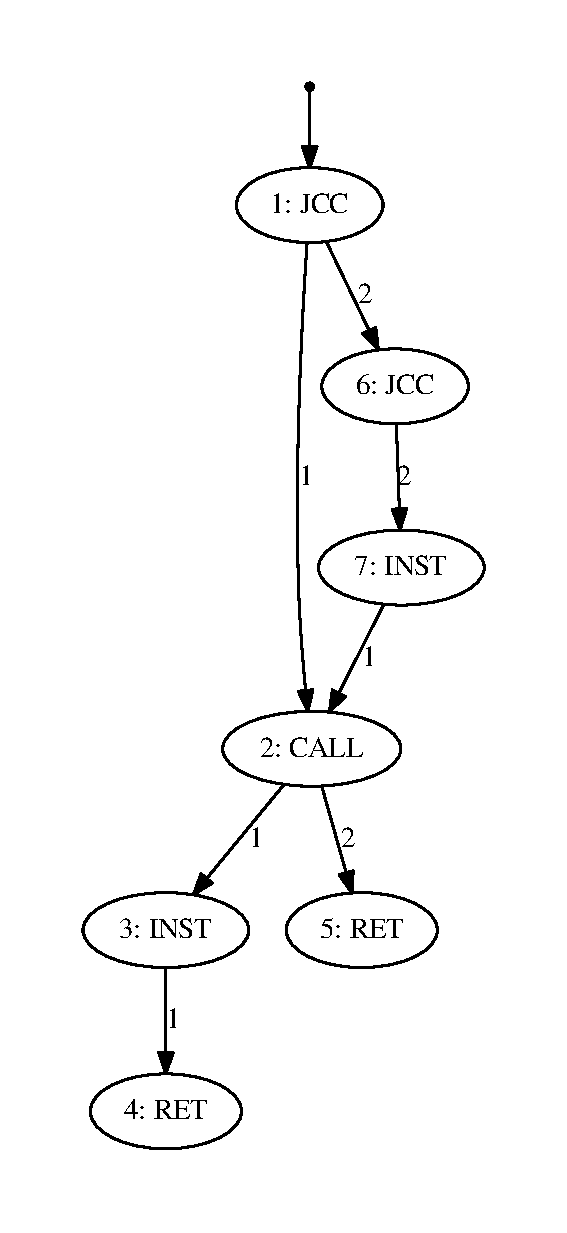
\includegraphics[height=0.4\textheight]{supports/algos/g1prof.pdf}}
\subfigure[]{
\label{fig:troisProf2}
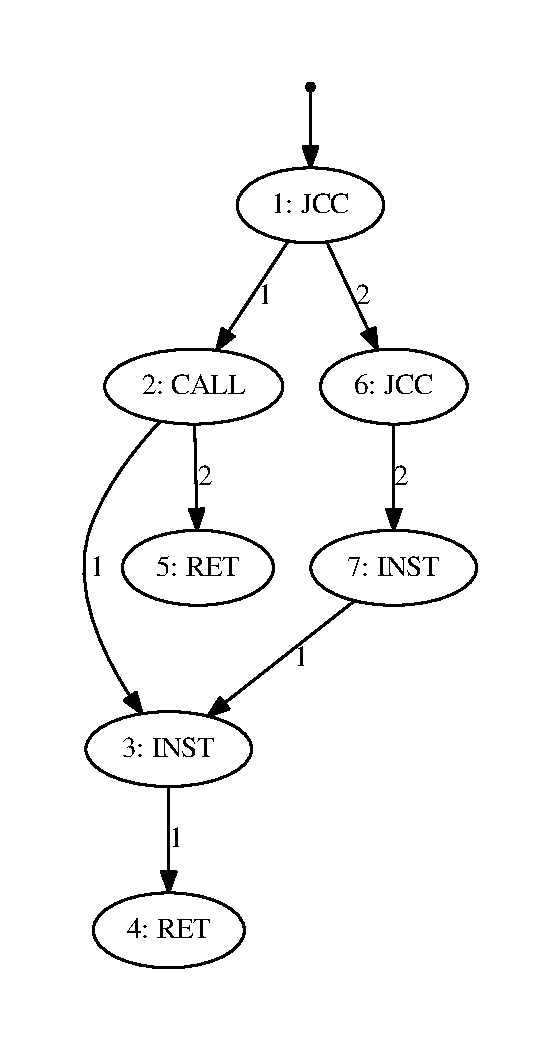
\includegraphics[height=0.4\textheight]{supports/algos/g2prof.pdf}}
\subfigure[]{
\label{fig:troisProf3}
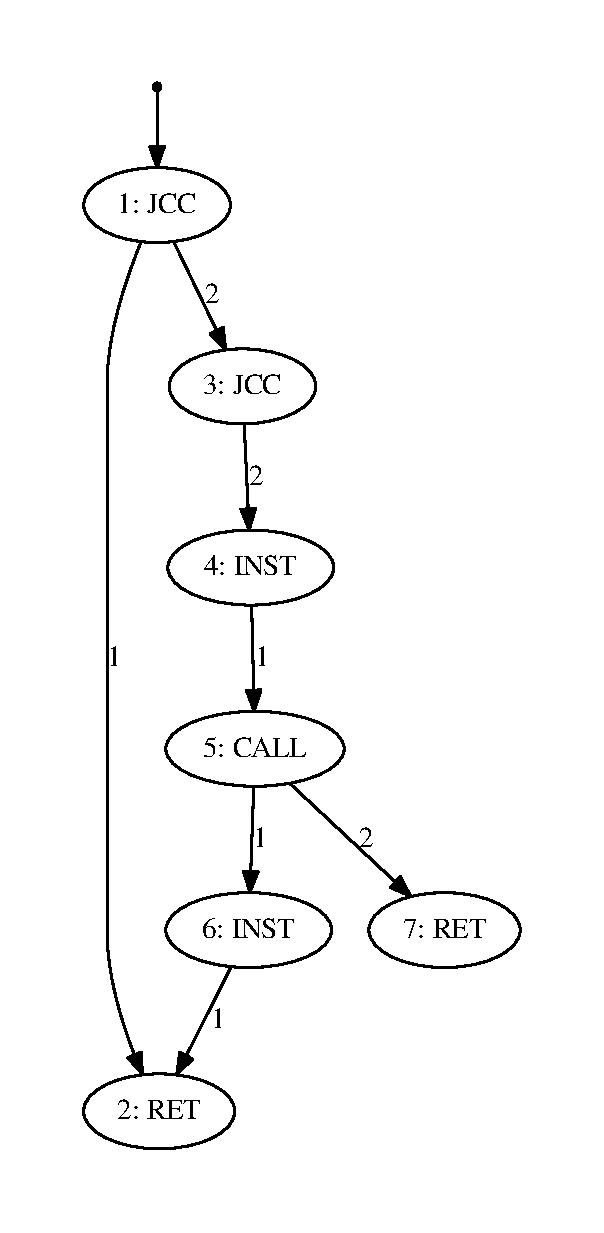
\includegraphics[height=0.4\textheight]{supports/algos/g3prof.pdf}}
\end{center}
\caption{Trois sites numérotés selon un parcours en profondeur}
\label{fig:troisProf}
\end{figure}
% $1: JCC\xrightarrow{1} 2: CALL \xrightarrow{1} 3: INST \xrightarrow{1} 4: RET \xrightarrow{R} 2 \xrightarrow{2} 5: RET \xrightarrow{R} 1 \xrightarrow{2} 6: JCC \xrightarrow{2} 7:INST \xrightarrow{1} 2$

\begin{figure}[h]
\begin{center}
\begin{tikzpicture}[
  tlabel/.style={pos=0.4,right=-1pt,font=\footnotesize\color{black!70!black} },
  every node/.style={color=black!25!black, circle, minimum size=6mm, draw=black!75, align=center},
  edge from parent/.style={draw=black!50,thick},
  level 1/.style={sibling distance=50mm, level distance=12mm},
]
\node[rectangle, rounded corners]{$racine$}
child {node {}
       child{node {}
	     child {node {}
	            child {node {}
		           child {node {}
		                  child {node {}
		                         child {node {}
		                                child {node {}
		                                       child {node {}
		                                              child {node {a}
								edge from parent node[tlabel,pos=0.2, left=15pt,draw=none] {$\xrightarrow{1} 2$}
		                                              }
		                                              child {node {b}
								edge from parent node[tlabel,pos=0.2, right=11pt,draw=none] {$\xrightarrow{1} 3$}
		                                              }
		                                              edge from parent node[tlabel,pos=0.3,draw=none] {$\xrightarrow{2} 7:INST$}
		                                       }
		                                       edge from parent node[tlabel,pos=0.3,draw=none] {$\xrightarrow{2} 6: JCC$}
		                                }
		                                edge from parent node[tlabel,pos=0.3,draw=none] {$\xrightarrow{R} 1$}
		                         }
		                         edge from parent node[tlabel,pos=0.3,draw=none] {$\xrightarrow{2} 5: RET$}
		                  }
		                  edge from parent node[tlabel,pos=0.3,draw=none] {$\xrightarrow{R} 2$}
		           }
		           edge from parent node[tlabel,pos=0.3,draw=none] {$\xrightarrow{1} 4: RET$}
	            }
	            edge from parent node[tlabel,pos=0.3,draw=none] {$\xrightarrow{1} 3: INST$}
	     }
	     edge from parent node[tlabel,pos=0.1, left=15pt,draw=none] {$\xrightarrow{1} 2: CALL$}
       }
       child{node {}
	     child {node {}
	            child {node {}
		           child {node {}
		                  child {node {}
		                         child {node {}
		                                child {node {}
		                                       child {node {}
		                                              child {node {c}
		                                              edge from parent node[tlabel,pos=0.3,draw=none] {$\xrightarrow{2} 7: RET$}
		                                              }
		                                              edge from parent node[tlabel,pos=0.3,draw=none] {$\xrightarrow{R} 5$}
		                                       }
		                                       edge from parent node[tlabel,pos=0.3,draw=none] {$\xrightarrow{1} 2$}
		                                }
		                                edge from parent node[tlabel,pos=0.3,draw=none] {$\xrightarrow{1} 6: INST$}
		                         }
		                         edge from parent node[tlabel,pos=0.3,draw=none] {$\xrightarrow{1} 5: CALL$}
		                  }
		                  edge from parent node[tlabel,pos=0.3,draw=none] {$\xrightarrow{2} 4: INST$}
		           }
		           edge from parent node[tlabel,pos=0.3,draw=none] {$\xrightarrow{2} 3: JCC$}
	            }
	            edge from parent node[tlabel,pos=0.3,draw=none] {$\xrightarrow{R} 1$}
	     }
	     edge from parent node[tlabel,pos=0.1, right=5pt,draw=none] {$~~~\xrightarrow{1} 2: RET$}
       }
       edge from parent node[tlabel,pos=0.5,draw=none] {$1: JCC$}
};
\end{tikzpicture}
\end{center}
\caption{Arbre de décision contenant les codages de sites de la figure \ref{fig:troisProf}}
\label{fig:arbreDecTarjan}
\end{figure}

\paragraph{Complexité.}
L'ajout d'un site à la base consiste à ajouter un codage de parcours dans l'arbre de décision, cette opération nécessite un nombre de comparaison en $W\times i$ où $i$ est le nombre de fils maximum de chaque sommet de l'arbre. Vu que les étiquettes des arcs de l'arbre sont de la forme $[\xrightarrow{\alpha}]i[:L]$, en notant $K$ le nombre de fils maximum de chaque sommet dans un site et $n_L$ le nombre d'étiquettes différentes pour les sommets des sites, $i\leq (K+2)\times W\times n_L$ soit $n=O(W)$ donc l'ajout d'un site à la base se fait en $O(W^2)$.

\subsubsection{Recherche d'un isomorphisme de sous-sites à partir de l'arbre de décision.}
Une fois l'arbre généré à partir de tous les codages des sites de $L_S$, on veut l'utiliser pour trouver tous les parcours de $L_S$ possibles dans le graphe de flot T. Pour compter le nombre de parcours de l'arbre que l'on peut réaliser à partir du sommet $r$ de $T$, on peut chercher à parcourir $T$ à partir de $r$ en parcourant les branches possibles dans l'arbre de décision. À chaque fois que l'on peut parcourir une branche jusqu'en bas c'est qu'un site isomorphe a été trouvé. L'algorithme \ref{algo:rechercheArbreTarjan} compte le nombre de ces branches possibles.

On peut utiliser cet algorithme pour retrouver tous les sous-sites isomorphes en utilisant l'algorithme précédent à partir de chaque sommet de $T$.

\begin{figure}[h]
\begin{algorithm}[H] %or another one check
\caption{Décompte, au sein d'un arbre de parcours donné, des parcours possibles d'un un graphe de flot, à partir d'un sommet donné}
\SetAlgoLined
\KwData{Un arbre A contenant les parcours de sites, un graphe de flot T, un sommet r de T}
\KwResult{Le nombre de parcours possibles}
\SetKwProg{Fn}{}{}{}
\SetKwFunction{FRecurs}{decompteSousSite}
\Return decompteSousSite(A, racine(A), T, r)\\
~\\

\Fn{\FRecurs{A, a, T, R}}{
  \eIf{a n'a aucun fils dans A}{
    \tcp{Si a n'a aucun fils, on a exactement décrit un parcours}
    \Return 1
  }
  {
    $somme\leftarrow 0$\\
    \For{f fils d'étiquette e de a dans A}{
	$(possible, s', T') \leftarrow etape(e, s, T)$\\
	\If{possible}{
	  $somme\leftarrow somme+decompteSousSite(A, f, T', s')$
	}
    }
  }
}

\SetKwProg{Fn}{}{}{}
\SetKwFunction{FRecurs}{etape}
\Fn(\tcp*[h]{L'étiquette e est de la forme $[\xrightarrow{\alpha}]i[:L]$}){\FRecurs{e, s, T}}{
  \eIf{e est de la forme $1:L$}{
    Numéroter le sommet s de T par 1.\\
    \Return (true, s, T)
  }
  {
    \tcp{Dans ce cas e est de la forme $\xrightarrow{\alpha}i[:L]$}
    \eIf{$\alpha$ est un entier k}{
    \uIf{s a un fils s' d'ordre k non numéroté dans T, d'étiquette L, et aucun sommet n'est numéroté i}{
    On numérote s' par i dans T.\\
    \Return $(true, s', T)$
    }
    \uElseIf{le sommet courant a un fils s' d'ordre k numéroté i}{
    \Return $(true, s', T)$
    }
    \Else{
    \tcp{Le parcours n'est pas possible si :\\ un autre sommet est déjà numéroté i,  ou\\ si le sommet à numéroter a déjà une autre numérotation,  ou\\ si l'étiquette n'est pas la bonne, ou\\ s'il n'y a pas de fils k}
    \Return $(false, s ,T)$
    }
    }
    {
      \tcp{Dans ce cas e est de la forme $\xrightarrow{R}i$}
      On note s' le sommet numéroté i dans T.\\
      \Return $(true, s', T)$
    }
  }
}
\label{algo:rechercheArbreTarjan}
\end{algorithm}
\end{figure}

\paragraph{Complexité.}
Dans le pire des cas il y a $n$ branches à l'arbre A qui partent de la racine où $n$ est le nombre de sites dans la base. Le parcours d'une branche avec au maximum un fils à chaque sommet, à partir de la racine se fait en $O(W)$ au vu de la récursion de l'algorithme \ref{algo:rechercheArbreTarjan}. Pour chercher les isomorphismes de sous-sites de $T$ il faut répéter l'opération pour chacun de ses sommets : la complexité totale dans le pire des cas pour résoudre le problème \ref{pbisosgbase} d'isomorphisme de sous-sites entre un graphe de flot et une base de sites est de $O(n.n_T.W)$. Ainsi on n'a pas amélioré la complexité dans le pire des cas par rapport à l'utilisation directe du parcours de Tarjan vu dans la section précédente, bien qu'en pratique l'algorithme soit plus rapide comme nous le verrons par la suite.

\FloatBarrier
\subsection{SIDT : Site Isomorphism Decision Tree}
Le problème \ref{pbisosg} consiste à détecter un site P dans un graphe de flot T. En pratique le site P aura été généré à partir d'un graphe de flot G. Si P est un sous-site de T, puisque l'on a généré le site à partir d'un parcours dans un autre graphe de flot, on peut envisager que le même parcours appliqué à T est susceptible de générer le site P. Ce n'est pas vrai dans le cas général et en ce sens l'algorithme présenté ici n'est pas complet.
Inversement il est clair que si le même parcours appliqué à partir de sommets de T et G génèrent le même site P, alors P est bien un sous-site de T.

On se propose donc, pour approcher la solution au problème \ref{pbisosg} de détection d'isomorphisme de sous-site entre un site P (généré par parcours avec un algorithme A à partir d'un sommet d'un graphe de flot G) et un graphe de flot T, de générer tous les sous-sites de T avec l'algorithme de parcours A et de regarder si P est dans cet ensemble.

Nous reprenons l'exemple de fonctionnement du détecteur par analyse morphologique décrit à la section \ref{sec:detecteur_morphologique}.
Le corpus est constitué du graphe de flot G et de sites P, donnés en figure \ref{fig:gfc_gf_P_sites}.
Afin de détecter le graphe de flot donné à la figure \ref{fig:gfc_gf_T_sites}, au lieu de vérifier si les sites P sont isomorphes à des sous-sites de T, nous découpons T en sites en suivant la même méthode que pour déterminer les sites à ajouter au corpus.
Nous comparons ensuite les sites générés à partir de T à ceux présents dans le corpus : il y a une correspondance si on trouve des sites identiques.
Ici nous voyons que les sites 1 et $\alpha$ sont identiques, ainsi que les sites 4 et $\epsilon$ et sont donc détectés par cette approche.
En revanche le site 3, pourtant sous-site de graphe T, n'est pas présent dans la liste des sites générés à partir de T par le parcours en largeur de taille limitée.

\begin{figure}[h]
\begin{center}
\def\imagetop#1{\vtop{\null\hbox{#1}}}
\begin{tabular}[t]{|c|c|}
\hline
Graphe de flot G & Signature : ensemble de sites P générés à partir de G\\
% \hline
\imagetop{\includegraphics[width=0.25\textwidth]{supports/algos/g1gf_cropped10.pdf}}
&
\imagetop{\includegraphics[width=0.6\textwidth]{supports/algos/g1_sites_cropped10.pdf}}
% &
% \imagetop{\includegraphics[width=0.2\textwidth]{supports/algos/g1_prof_cropped10.pdf}}
\\
\hline
\end{tabular}
\end{center}
\caption{Graphe de flot d'un programme et sa signature dans le corpus}
\label{fig:gfc_gf_P_sites}
\end{figure}

\begin{figure}[h]
\begin{center}
\def\imagetop#1{\vtop{\null\hbox{#1}}}
\begin{tabular}[t]{|c|c|}
\hline
Graphe de flot de test T & Ensemble de sites générés à partir de T\\
% \hline
\imagetop{\includegraphics[width=0.25\textwidth]{supports/algos/g1p_cropped10.pdf}}
&
\imagetop{\includegraphics[width=0.7\textwidth]{supports/algos/g1p_sites_cropped10.pdf}}
% &
% \imagetop{\includegraphics[width=0.2\textwidth]{supports/algos/g1_prof_cropped10.pdf}}
\\
\hline
\end{tabular}
\end{center}
\caption{Graphe de flot d'un programme de test et son découpage en sites}
\label{fig:gfc_gf_T_sites}
\end{figure}

Pour régler le problème \ref{pbisosgbase} de détection d'un site dans une base de graphes de flot, on va créer un arbre de décision contenant tous les sites générés à partir du parcours en largeur des graphes de flot de la base.

\subsubsection{Arbre de décision pour la détection de sites}
Chaque site est généré par un parcours numérotant ses sommets, et chaque sommet a un nombre de fils bornés. On représente alors les sites sous forme matricielle : chaque ligne représente un sommet, le premier élément de la colonne est l'étiquette du sommet et les éléments suivants sont les numéros des fils de ce sommet (0 indique qu'il n'y a pas de sommet). La représentation des sites de la figure \ref{fig:troisProf} est donnée figure \ref{fig:troisProfMatRed}.

\begin{figure}[h]
\begin{center}
\subfigure[]{
\label{fig:troisProfMatRed1}
$\begin{array}{r|ccc} Sommet & Etiquette & Fils 1 & Fils 2 \\
\hline
1 & JCC & 2 & 6\\
2 & CALL & 3 & 5\\
3 & INST & 4 & 0\\ 
4 & RET & 0 & 0\\ 
5 & RET & 0 & 0\\ 
6 & JCC & 0 & 7\\ 
7 & INST & 2 & 0\\ 
\end{array}$
}
\subfigure[]{
\label{fig:troisProfMatRed2}
$\begin{array}{r|ccc} Sommet & Etiquette & Fils 1 & Fils 2 \\
\hline
1 & JCC & 2 & 6\\
2 & CALL & 3 & 5\\
3 & INST & 4 & 0\\ 
4 & RET & 0 & 0\\ 
5 & RET & 0 & 0\\ 
6 & JCC & 0 & 7\\ 
7 & INST & 3 & 0\\ 
\end{array}$
}
\subfigure[]{
\label{fig:troisProfMatRed3}
$\begin{array}{r|ccc} Sommet & Etiquette & Fils 1 & Fils 2 \\
\hline
1 & JCC & 2 & 3\\
2 & RET & 0 & 0\\
3 & JCC & 0 & 4\\ 
4 & INST & 5 & 0\\ 
5 & CALL & 6 & 7\\ 
6 & INST & 2 & 0\\ 
7 & RET & 0 & 0\\ 
\end{array}$
}
\end{center}
\caption{Représentation matricielle des sites de la figure \ref{fig:troisProf}}
\label{fig:troisProfMatRed}
\end{figure}

Un site généré par un parcours a une unique représentation sous cette forme parce que, d'une part, le parcours a numéroté ses sommets qui sont donc ordonnés ; d'autre part les fils de chaque sommet sont numérotés, enlevant toute ambiguïté sur l'ordre à donner aux fils dans la matrice générée.

On peut ensuite agréger tous les sites générés dans un arbre de décision (figure \ref{fig:arbreDecTarjan}).

\begin{figure}[h]
\begin{center}
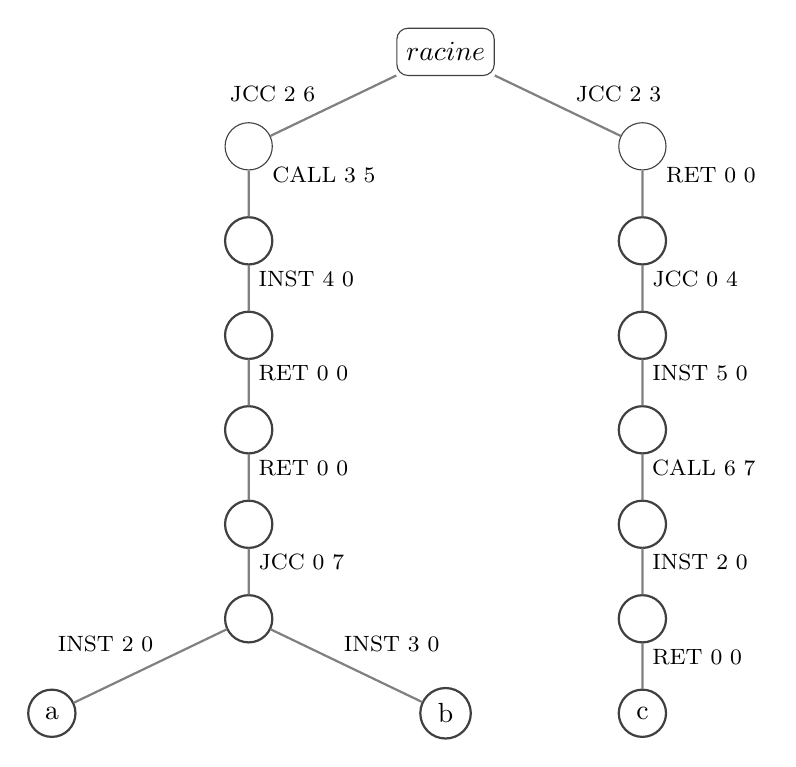
\begin{tikzpicture}[
  tlabel/.style={pos=0.4,right=-1pt,font=\footnotesize\color{black!70!black} },
  every node/.style={color=black!25!black, circle, minimum size=6mm, draw=black!75, align=center},
  edge from parent/.style={draw=black!50,thick},
  level 1/.style={sibling distance=50mm, level distance=12mm},
]
\node[rectangle, rounded corners]{$racine$}
child{node{}
      child{node {}
	     child {node {}
	            child {node {}
		           child {node {}
		                  child {node {}
		                         child {node {a}
		                                edge from parent node[tlabel,pos=0.2, left=10pt,draw=none] {INST 2 0}
		                         }
		                         child {node {b}
		                                edge from parent node[tlabel,pos=0.2, right=12pt,draw=none] {INST 3 0}
		                         }
		                         edge from parent node[tlabel,pos=0.3,draw=none] {JCC 0 7}
		                  }
		                  edge from parent node[tlabel,pos=0.3,draw=none] {RET 0 0}
		           }
		           edge from parent node[tlabel,pos=0.3,draw=none] {RET 0 0}
	            }
	            edge from parent node[tlabel,pos=0.3,draw=none] {INST 4 0}
	     }
	     edge from parent node[tlabel,pos=0.1, right=5pt,draw=none] {CALL 3 5}
       }
       edge from parent node[tlabel,pos=0.3,left=10pt,draw=none] {JCC 2 6}
      }
child {node {}
       child{node {}
	     child {node {}
	            child {node {}
		           child {node {}
		                  child {node {}
		                         child {node {c}
		                                edge from parent node[tlabel,pos=0.3,draw=none] {RET 0 0}
		                         }
		                         edge from parent node[tlabel,pos=0.3,draw=none] {INST 2 0}
		                  }
		                  edge from parent node[tlabel,pos=0.3,draw=none] {CALL 6 7}
		           }
		           edge from parent node[tlabel,pos=0.3,draw=none] {INST 5 0}
	            }
	            edge from parent node[tlabel,pos=0.3,draw=none] {JCC 0 4}
	     }
	     edge from parent node[tlabel,pos=0.1, right=5pt,draw=none] {RET 0 0}
       }
       edge from parent node[tlabel,pos=0.3,right=12pt,draw=none] {JCC 2 3}
};
\end{tikzpicture}
\end{center}
\caption{Arbre de décision contenant les matrices de la figure \ref{fig:troisProfMatRed}}
\label{fig:arbreDecSIDT}
\end{figure}

\paragraph{Complexité.}
L'apprentissage d'un site nécessite le parcours d'au plus W éléments de l'arbre de décision. Chaque sommet de l'arbre de décision a au plus $n_L.W.W$ fils où $n_L$ est le nombre d'étiquettes possibles. L'apprentissage d'un site se fait donc en $O(W^3)$ où W est le nombre de sommets des sites à apprendre.

\subsubsection{Recherche d'un isomorphismes de sous-sites}
Rechercher un isomorphisme de sous-sites à partir de l'arbre de décision ainsi créé revient à écrire le site sous forme matricielle et à faire une recherche dans l'arbre de décision.

\paragraph{Complexité.}
La complexité de la recherche d'un site dans l'arbre de décision est la même que pour l'ajout dans d'un site dans l'arbre et se fait en $O(W^3)$. 


\section{Comparaison des performances}
\subsection{Complexité}

On dispose donc de quatre algorithmes à comparer : celui par recherche exhaustive avec les matrices d'adjacence, l'algorithme d'Ullmann, pris pour référence, l'algorithme de Tarjan avec arbre de décision et l'algorithme incomplet par arbre de décision (SIDT).
Nous calculons les complexités dans le pire des cas de l'ajout d'un graphe de flot dans la base et d'analyse d'un graphe de flot inconnu.
On dispose donc d'une part d'un corpus de programmes dont les graphes de flot ont été déterminés.
Nous notons :
\begin{itemize}
%  \item $m$ le nombre de programmes du corpus.
%  \item $n_M$ le nombre maximal de sommets des graphes de flot du corpus.
 \item $S$ le nombre de sites du corpus.
 \item $n$ le nombre de sommets du graphe de flot que l'on cherche à ajouter ou analyser.
 \item $W$ le nombre de sommets des sites de la base (constante fixée typiquement entre 12 et 24).
 \item $h$ la constante introduite à la section \ref{sec:ullmann_complexite} sur l'algorithme d'Ullmann, comprise entre 0 et 1, dépendant de la répartition des étiquettes, et évaluée à $0.34$.
 \item $k$ la valence maximale dans les graphes de flot de contrôle, c'est à dire le nombre maximum de fils qu'un sommet peut avoir ; $k=2$.
\end{itemize}
D'autre part nous étudions deux opérations sur cette base.
La première est l'ajout d'un graphe de flot, à $n$ sommets, à cette base de reconnaissance.
La seconde est l'analyse d'un graphe de flot inconnu, comprenant $n$ sommets.
Il y donc $S$ sites de taille $W$ dans la base.

La complexité pour déterminer tous les sites d'un graphe de flot à $n$ sommets est $O(n.(k+1).W)$.
Ainsi la complexité de l'ajout pour l'algorithme par parcours est $O(n.(k+1).W+n.W^2)$, soit $O(n)$.
De même l'analyse d'un graphe de flot a pour complexité $O(n.(k+1).W+S.n.W)$, soit $O(S.n)$

La complexité de l'ajout pour SIDT est $O(n.(k+1).W+n.W^3)$=$O(n)$ et celle pour l'analyse est $O(n.(k+1).W+n.W^3)$=$O(n)$.

\paragraph{Complexité totale.}
Si l'on ne considère aucune variable comme constante, la complexité totale de chacun des algorithmes pour ces opérations est donnée par le tableau donné en figure \ref{fig:complexite_1}.
Les deux premiers algorithmes ne rangent les pas sites dans une base spécifique ; on dispose simplement d'une liste de sites que l'on doit générer à partir du graphe de flot.

\begin{figure}[h]
\begin{center}
\begin{tabular}{|c|c|c|}
 \hline
 Algorithme & Ajout d'un graphe de flot & Analyse d'un graphe de flot\\
 \hline
 Recherche exhaustive & $O(n.W)$ & $O(S.n^3.n!)$\\
 Ullmann & $O(n.W)$ & $O(S.(n.h)^W)$ \\
 Parcours & $O(n.W^3)$ & $O(S.n.W)$\\
 SIDT & $O(n.W^3)$ & $O(n.W^3)$\\
 \hline
\end{tabular} 
\end{center}
\caption{Complexité totale}
\label{fig:complexite_1}
\end{figure}

Par la suite nous exploiterons le fait que $W$ et $h$ sont des constantes.

\paragraph{Complexité à nombre de sites dans la base constant.}
Nous fixons le nombre de site dans le base, $S$.
La complexité de l'ajout et de l'analyse devient celle donnée en figure \ref{fig:complexite_2}.

\begin{figure}[h]
\begin{center}
\begin{tabular}{|c|c|c|}
 \hline
 Algorithme & Ajout d'un graphe de flot & Analyse d'un graphe de flot\\
 \hline
 Recherche exhaustive & $O(n)$ & $O(n^3.n!)$\\
 Ullmann & $O(n)$ & $O(n^W)$ \\
 Parcours & $O(n)$ & $O(n)$\\
 SIDT & $O(n)$ & $O(n)$\\
 \hline
\end{tabular} 
\end{center}
\caption{Complexité à $W$, $P$ et $S$ fixés}
\label{fig:complexite_2}
\end{figure}

Ce tableau nous indique que, bien que l'on ait grandement réduit la complexité initiale de l'algorithme d'Ullmann, l'utilisation de l'un des deux premiers algorithmes augmente en complexité d'un facteur d'au moins $n^{12}$ avec la taille du graphe à analyser.

Les deux autres algorithmes ont eux une complexité augmentant linéairement avec la taille du graphe à ajouter ou à analyser.

\paragraph{Influence de la taille de la base.}
Les trois premiers algorithmes ont, pour l'analyse de graphe de flot inconnu, une complexité linéaire en le nombre de site de la base, $S$.
L'algorithme SIDT est le seul pour lequel le temps de l'analyse ne dépend pas du nombre de sites dans la base, ce qui le rend à même de mieux gérer un corpus de grande taille.

% \begin{center}
% \begin{tabular}{|c|c|c|}
%  \hline
%  Algorithme & Ajout d'un graphe de flot G & Analyse d'un graphe de flot T\\
%  \hline
%  Recherche exhaustive & (pas de base) & $O(S.n^3.n!)$\\
%  Ullmann & (pas de base) & $O(S.n^W)$ \\
%  Tarjan & $O(n)$ & $O(S.n^2)$\\
%  SIDT & $O(n)$ & $O(n)$\\
%  \hline
% \end{tabular} 
% \end{center}

% Du point de vue de la complexité dans le pire des cas, il est donc clair que les deux premiers algorithmes sont très inefficaces et l'algorithme SIDT devrait s'avérer être le plus rapide avec une complexité constante lors de l'agrandissement de la base, linéaire seulement en la taille du graphe de flot de contrôle ajouté ou analysé.

% \begin{center}
% \begin{tabular}{|c|c|c|}
%  \hline
%  Algorithme & Ajout d'un graphe de flot G & Analyse d'un graphe de flot T\\
%  \hline
%  Recherche exhaustive & (pas de base) & $O(S)$\\
%  Ullmann & (pas de base) & $O(S)$ \\
%  Tarjan & $O(1)$ & $O(S)$\\
%  SIDT & $O(1)$ & $O(1)$\\
%  \hline
% \end{tabular} 
% \end{center}

\subsection{Détail des implémentations}
Nous avons implémenté différents algorithmes de la manière suivante. Ils prennent en entrée un ou plusieurs graphes de flot à insérer dans la base de programmes connus et un ou plusieurs graphes de flot à tester.
Le programme donne en sortie, pour chaque graphe de flot à tester, les correspondances trouvées avec ceux ajoutés à la base.
Les graphes de flot sont stockés dans des fichiers binaires ou des fichiers de graphes (\texttt{.dot}).

\paragraph{Algorithme d'Ullmann.}
Développé en 2000 lignes C, l'implémentation offre les différentes options d'optimisation dont celles discutées précédemment à la section \ref{sec:ullmann_optimisation}.
Elle est principalement constituée des deux fonction \emph{backtrack} et \emph{forwardChecking}.

\paragraph{Arbre de décision avec algorithme de Tarjan.}
Développée en 500 lignes python, l'implémentation permet d'enregistrer la base dans un fichier pour effectuer l'analyse à partir d'une base existante.

\paragraph{SIDT.}
Développée en 1200 lignes de C, l’implémentation permet de créer une base mais pas de l'enregistrer.

\subsection{Performance des implémentations}
[à faire : avec un échantillon pour la base, un pour les tests, mesure de performances en temps mais aussi en précision entre SIDT et Tarjan/Ullmann]
